\documentclass[12pt,a4paper,twoside,spanish]{book}

\usepackage{Formato}

\title{Tesis 4 Posicionamiento de pacientes virtuales}
\author{Aaron Sújar}

%%%%%%%%%%%%%%%%%%%%%%%%%%%%%%%%%%%%%%%%%%%%
%Nuevos comandos
%%%%%%%%%%%%%%%%%%%%%%%%%%%%%%%%%%%%%%%%%%%%
%\usepackage[normalem]{ulem}
%\usepackage{color}
%\usepackage[margin=2in]{geometry}
%\usepackage{todonotes}
\newcommand{\del}[1]{\textcolor{red}{\sout{#1}}} %\sout}
\newcommand{\new}[1]{\textcolor{blue}{\uline{#1}}} %\sout}

\begin{document}
\frontmatter

\thispagestyle{empty}
\chapter*{Acronyms}

\begin{acronym}
\acro{B-rep}{representación superficial}
\acro{Bangor}{Bangor University}
\acro{DQS}{dual quaternion skinning}
\acro{CAD}{diseño asistido por computador}
\acro{COR}{centros de rotación}
\acro{Courseware}{aplicación de entrenamiento}
\acro{DICOM}{Imagen y Comunicación Digital en Medicina}
\acro{DOF}{grados de libertad}
\acro{E/S}{Entrada/Salida}
\acro{EASA}{Agencia Europea de Seguridad Aérea}
\acro{FEM}{método de elementos finitos}
\acro{FORTH}{Foundation for Research and Technology - Hellas}
\acro{CGAL}{Computational Geometry Algorithms Library}
\acro{GLSL}{OpenGL Shading Language}
\acro{GMRV}{Grupo de Modelado y Realidad Virtual}
\acro{GPL}{GNU General Public License}
\acro{GPU}{unidad de procesamiento gráfico}
\acro{ITGVPH}{Integrated Toolkit for Generation of VPH Models}
\acro{INRIA}{Institut National de Recherche en Informatique et en Automatique}
\acro{IRM}{imagen por resonancia magnética}
\acro{IU}{interfaz de usuario}
\acro{joints}{articulaciones virtuales}
\acro{kvp}{tensión de pico}
\acro{kV}{kilovoltio}
\acro{keV}{kiloelectronvoltio}
\acro{LGPL}{GNU Lesser General Public License}
\acro{LBS}{linear blending skinning}
\acro{mAs}{miliamperio por segundo}
\acro{MoCap}{captura de movimientos}
\acro{RA}{anestesia regional}
\acro{RAAs}{Regional Anaesthesia Assistant}
\acro{RAM}{Random Access Memory}
\acro{RASim}{Regional Anaesthesia Simulator}
\acro{RASimAs}{Regional Anaesthesia Simulator and Assistant}
\acro{RDT}{triangulación restringida de delaunay}
\acro{RV}{realidad virtual}
\acro{RWTH}{RWTH Aachen University}
\acro{SBS}{Spherical Blend Skinning}
\acro{SINTEF}{Stiftelsen for industriell og teknisk forskning}
\acro{SG}{Sensegraphics}
\acro{SOFA}{Simulation Open Framework Architecture}
\acro{TASMIP}{TASMIP}{tungsten anode spectral model using interpolating polynomials}
\acro{TC}{tomografía axial computarizada}
\acro{TPTVPH}{Toolkit for Pose Transforms of VPH Models}
\acro{tracker}{dispositivo de seguimiento}
\acro{tabla hash}{Spatial Hash Table}
\acro{UKA-IMI}{Department of Medical Informatics: Uniklinik RWTH Aachen}
\acro{URJC}{Universidad Rey Juan Carlos}
\acro{US}{ultrasonidos} 
\acro{ViSTA}{Virtual Reality Toolkit}
\acro{VPH}{pacientes virtuales}
\acro{VTU}{formato de Visualization Toolkit}
\acro{WP}{paquetes de trabajos}
\acro{X3D}{formato Extensible 3D}
\acro{XML}{Extensible Markup Language}
\acro{ZPD}{zona de desarrollo próximo}


\end{acronym}



\tableofcontents
\listoffigures
 
\listoftables
\mainmatter
\chapter{Posicionamiento de pacientes virtuales} 
\label{cap:posing}

En este capítulo, se propone un método que permite adaptar la anatomía, interna y/o externa, de un modelo anatómico virtual a cualquier pose requerida. Tal y como se explica en la capítulo de introducción \ref{cap:intro}, esta tesis se ha desarrollado en el contexto del proyecto \ac{RASimAs}, financiado por el 7º programa marco de la Unión Europea. Crear un simulador de anestesia regional que permitiese entrenar a los futuros médicos fue uno de los principales objetivos del proyecto. 
Este simulador debía ofrecer una amplia base de pacientes virtuales, de forma que el anestesista se pudiese enfrentar a una gran diversidad de variedades anatómicas durante su aprendizaje. Dependiendo del nervio que se desee bloquear, el procedimiento requiere una pose especifica del paciente. Los algoritmos, que aquí se describen, se diseñaron para adaptar los modelos anatómicos de la base de datos de pacientes a las poses requeridas en las distintas versiones del procedimiento. Dada su importancia, \ac{RASimAs} dedicó una tarea completa a solucionar esté problema (ver sección \ref{art:rasimas}). 
De esta forma, los requisitos que guiaron su diseño vienen impuestos por las necesidades del proyecto (ver sección \ref{posing:req}). Todos los algoritmos propuestos se integraron en la herramienta \ac{TPTVPH}, desarrollada completamente en el contexto de esta tesis y que formaba parte de la \emph{suite}\footnote{Paquete de aplicaciones desarrolladas con distintos objetivos y capaces de cooperar entre sí.} de aplicaciones (\ac{ITGVPH}), módulo de creación de pacientes virtuales de  \ac{RASimAs}.

%\del{Como se puede leer en el capítulo de introducción \ref{cap:intro}, el objetivo de esta tesis viene influenciado por el proyecto europeo \ac{RASimAs} cuya finalidad de crear un simulador de anestesia que pueda entrenar con una base de datos de pacientes virtuales consiguiendo variabilidad anatómica adecuada para practicar el procedimiento.
%El proyecto europeo dedica una tarea completa a solucionar la problemática de poder reposicionar modelos anatómicos con el objetivo de crear una base de datos con una gran variabilidad anatómica (ver sección \ref{art:rasimas}).}

%\todo{No está mal escrito, pero es redundante con los objetivos de RASimAs}
%\del{En el contexto de entrenamiento médico, es fundamental que los usuarios se enfrenten a la mayor cantidad de situaciones posibles. 
%Es por ello, que se ha propuesto un método que permita la creación de un conjunto de datos extenso de forma automática o semi-automática y a la vez pueda ser utilizada en cualquier simulador de realidad virtual.}

El conjunto de algoritmos, que se han diseñado a lo largo de este trabajo de tesis, extienden la animación esqueletal clásica a la animación de los tejidos internos de un modelo virtual. Al tratarse de un método puramente geométrico ofrece, con un coste computacional bajo, resultados plausibles y estables. Otro de los motivos principales por los que se escogió un método geométrico frente a un método basado en modelos fiscos, es la posibilidad de manipular modelos anatómicos incompletos o de los que no se dispone de propiedades mecánicas. Estas características, hacen que su uso sea adecuado en otras aplicaciones, incluso más allá del ámbito médico.  En el mundo del ocio interactivo, especialmente en el sector de los videojuegos, un bajo coste computacional, la estabilidad, la plausibilidad de los resultados y la posibilidad de aplicarlo a estructuras anatómicas incompletas, son características más importantes que la precisión física de las transformaciones. 

%\todo{hay que dar mas peso a lo de los modelos incompletos que a la interactividad. En el caso de rasimas es más importante. }
%\del{ Con este propósito, se han diseñado y adaptado diferentes algoritmos de animación esqueletal con el objetivo de animar tejidos internos y externos de un paciente virtual. Se ha elegido utilizar métodos geométricos que permiten la creación de resultados plausibles y a la vez tienen la ventaja de que permiten una deformación interactiva. Esta ventaja frente a los métodos basados en físicos dan lugar a que el algoritmo presentado en este capítulo pueda incluirse en cualquier simulador que requiera de deformación en tiempo real. Otra ventaja que tiene el método propuesto es la posibilidad de manipular modelos anatómicos incompletos o que no se disponen de sus propiedades mecánicas.}

\section{Requisitos de diseño}
\label{posing:req}
%\new{Decisiones de diseño}

%\todo{De manera ideal no son los requisitos nos los fijan los socios. Sino los objetivos del proyecto. Lo cambiamos a decisiones? }
%\del{Al formar parte de un proyecto donde intervienen más grupos de investigación, la tarea específica viene acompañada de una serie de requisitos que necesitan ser respetados, pero al mismo tiempo es la principal motivación que se encuentra al formular una solución innovadora:}
En las etapas iniciales del proyecto \ac{RASimAs} se establecieron los objetivos del módulo de creación de pacientes virtuales, del que la herramienta \ac{TPTVPH} formaba parte. A partir de dichos objetivos se definieron los requisitos de \ac{TPTVPH} y por ende de los algoritmos que debían ser diseñados.


%\todo {0.No está escrito como unos requisitos. Mezclas requisitos con decisiones de diseño!!!
%1. El enfoque geométrico no es una recomendación es una consecuencia de los objetivos
%2. Realmente en el estado del arte, se ha demostrado que el enfoque geométrico es menos sensible a la calidad de datos de entrada?????. 
%3. a que te refieres con tipos de datos. Realmente te refieres a modelos incompletos. }
\begin{itemize}
    \item El proceso de selección de poses deberá ser guiado y supervisado por un experto para garantizar la validez de los modelos generados. Dado el coste económico del tiempo de un experto, la herramienta deberá tener una interfaz sencilla y los algoritmos deberán ejecutarse en modelos complejos con tasas de refresco interactivas.
    \item La intervención del usuario se limitará a la selección de la pose final. El resto de procesos involucrados en la preparación de los modelos deberán realizarse de forma automática.
    \item Los datos de entrada se obtendrán promediando datos de diferentes pacientes reales y registrándolos sobre el modelo de \emph{ZygoteBody}$^{TM}$ \cite{kelc2012zygote}. Los datos de pacientes reales provendrán distintas técnicas de imagen médicas (\ac{US}, \ac{IRM}, \ac{TC}). Dado que no existe ninguna técnica de imagen capaz de capturar todas las estructuras anatómicas internas, los pacientes virtuales generados no dispondrán de modelos de todos sus tejidos internos. Solo se garantiza que se dispondrán de modelos adecuados de piel y huesos. 
    \item En el momento de realizar el posicionamiento del paciente virtual, no se conocerán las propiedades mecánicas de las distintas estructuras anatómicas que lo componen.
    % \todo{Te lo he rescrito porque creo que me suena raro. Creo que no resaltas lo que es realmente importante. Aaron: Me gustaba lo de generar colisiones adicionales... }
     %\del{Para mantener la calidad del modelo anatómico de las siguientes etapas y tareas dependientes de esta (p. ej. el módulo de \ac{US}), el resultado de este algoritmo no deberá generar colisiones adicionales indeseables entre los tejidos y tener igual o menos colisiones que las existentes al llegar como entrada.}
    \item Los algoritmos propuestos deberán evitar que se produzcan autocolisiones o colisiones entre los distintos tejidos, dado que esto podría provocar fallos en  algunos módulos del simulador. El modulo de \ac{US} es especialmente sensible a estos artefactos.
     %\item \del{Se recomienda un enfoque geométrico ya que, en fases previas al proyecto, se consideró la posibilidad de utilizar un método basado en físicas para la tarea en cuestión. Como se ha podido comprobar en el estado del arte \ref{art:animation}, un enfoque geométrico es menos dependiente de la calidad de los datos de entrada, obtenidos por etapas anteriores en este proyecto. Un modelo basado en físicas necesitaría una descripción completa de todos los tejidos; sin embargo, el método geométrico puede ser útil si estos datos no están disponibles.}
    %\item  \del{\ac{TPTVPH} (ver sección \ref{art:rasimas}) podrá ser capaz de trabajar con cualquier tipo de datos que procedan de un paciente virtual. Como no se puede asegurar que todos los tejidos se encuentren disponibles, el algoritmo deberá ser lo máximo flexible posible para manejarlos.}
    
    %\item \todo{He usado este objetiv para meter la importancia de la interactividad.}\del{Aun así, el proceso de posicionamiento tendrá que ser supervisado. Profesionales cualificados definirán un conjunto genérico de posturas para el procedimiento de \ac{RA}. Un método semiautomático será desarrollado para facilitar la consecución de la validez y calidad de los modelos de pacientes virtuales.}
    %\item \del{El usuario podrá modificar la postura del \ac{VPH} a través de una interfaz 3D interactiva \del{con la intención de reducir el procedimiento completo}. El algoritmo deberá ejecutar en tiempo real para mejorar la experiencia de uso. }
    
 \end{itemize}


%\todo{No puede haber solo una subsección!!!}
%\subsection{Requisitos del posicionador de pacientes virtuales}

%\todo{Si te sobra tiempo, puede describir las ventajas de los métodos fiscos sobre los geométricos. Coste computacional, estabilidad, flexibilidad. Por otro lado, los cambios de poses requieren grandes movimientos que para ser capturados de forma precisa necesitan que se tengan en cuenta numerosos comportamientos que no fáciles de simular (deformaciones elásticas, interacciones:  deslizamientos, contactos). Requieren modelos completos y bien caracterizados... }

En un primer momento, se planteó la posibilidad de trabajar con técnicas basadas en modelos físicos en aras de conseguir un deformación precisa de los tejidos. Esta opción fue desechada principalmente por no disponer de una descripción mecánica de los tejidos involucrados en la simulación. Estás técnicas generalmente requieren importantes recurso computacionales que impiden que puedan usarse en aplicaciones interactivas. El problema se agrava cuando se quieren simular grandes deformaciones que involucran diversos y complejos fenómenos físicos.

Por otro lado, muchas veces la resolución de los sistemas de ecuaciones diferenciales que modelan el comportamiento del sistema requiere de métodos numéricos que no siempre son estables. En experimentos iniciales se optó por utilizar técnicas muy utilizadas como las propuestas en  \cite{Muller2004} e implementadas en \ac{SOFA}. Pronto quedó patente que los modelos de tejidos utilizados eran demasiado complejos como para que este tipo de técnicas funcionasen de forma adecuada.
%\del{Como se puede leer en la sección \ref{art:animation}, estos métodos basaban sus resultados en un alto coste computacional, o en centrarse en una única anatomía.  Además, algunas técnicas requieren de modelos muy bien caracterizados o de capturas en diferentes posiciones, lo cual es el principal objetivo que quiere solventar la herramienta planteada. Técnicas clásicas como \cite{Muller2004}, se ejecutaron en el software de simulación \ac{SOFA}. Los modelos iniciales del sistema eran demasiado complejos para conseguir tasas de refresco adecuadas para una interacción con el usuario.}
Durante el desarrollo de esta tesis, se han propuesto nuevas técnicas que podrían cumplir con algunos de los requisitos planteados (ver sección \ref{art:fisica}). En \cite{abu2015position}, se propone un método capaz de simular el comportamiento interno de la anatomía, \new{permitiendo la caracterización mecánica de los tetraedros según el tejido anatómico al que pertenecen.}  \del{con el objetivo de generar movimientos de los tejidos óseos plausibles}\todo{No entiendo que quiere decir: -- se puede asignar propiedades mecánicas diferenteas a cada tetraedro.}. El principal inconveniente de esta técnica es la imposibilidad de conseguir tiempos interactivos con la complejidad de los modelos anatómicos que se estaban utilizando. \new{Además, la publicación de este artículo ha sido posterior a la fecha de incorporación del algoritmo en el proyecto europeo.}\todo{Yo reescribiria la última frase es muy enrevesada}\del{, además de tener en cuenta que su aparición fue posterior a la fecha de finalización de la tarea.}

Como consecuencia de lo expuesto, se decidió desechar la opción de trabajar con métodos basados en modelos físicos y se optó por diseñar una técnica geométrica. En las siguientes secciones se describirá el método propuesto.
%%%%%%%%%%%%%%%%%%%%%%%%%%%%%%%%%%%%%%%%%%%%%%%%%%%%%%%%%
\section{Algoritmo propuesto}
\label{posing:method}
%%%%%%%%%%%%%%%%%%%%%%%%%%%%%%%%%%%%%%%%%%%%%%%%%%%%%%%%%
%\todo{1. Indicar muy brevemente las ventajas de la animación esqueletal alineadas con los objetivos. 2. Indicar porque la técnica clásica no se puede utilizar. La extendemos para anatomía interna. 3. No usamos las técnicas clásicas porque no tiene en cueta la anatomía interna. %2. No entiendo la seguna parte de la frase}
En este apartado, se propone un conjunto de técnicas capaces de animar la anatomía interna y externa de un paciente virtual. El cauce de animación, que aquí se describe, fue diseñado para trabajar con \acs{B-rep}s de los distintos tejidos, aunque dada la flexibilidad del enfoque planteado, posteriormente se extendió a otro tipo de representaciones (ver sec. \ref{posing:animvol}). 
\todo{
%mete la referencia. Lo he contado por que tú lo haces pero no se si es el mejor sito. 
Tienes que ir soltando las ideas una a una, no todas a la vez. }
%
%\del{El objetivo es ser capaz de modificar toda la anatomía interna y externa de un modelo anatómico virtual usando una representación superficial. En el mundo de los gráficos por computador, tradicionalmente, se ha utilizado la animación esqueletal para \new{animar modelos articulados}. ????????????????????????????????? Aunque permite una animación de modelos complejos en tiempo interactivo, no tiene en cuenta la relación espacial entre tejidos. Por esta razón, se ha diseñado un cauce basado en la animación esqueletal que se extiende para el uso de representaciones volumétricas.????}
\todo{%Lo reescribo yo!. Todo esto es muy confuso. 
No hay un hilo conductor ni una idea clara que vender} 

En el mundo de los gráficos por computador, tradicionalmente\del{,} se ha utilizado la animación esqueletal para animar modelos articulados, dado que produce resultados visualmente plausibles y son muy eficientes desde el punto de vista computacional. Este conjunto de técnicas se basan en asignar un esqueleto virtual a la representación poligonal de la superficie de un modelo 3D. \new{Es conveniente} Destacar que un esqueleto virtual no es más que un conjunto jerárquico de huesos virtuales donde los puntos de rotación de cada hueso se define localmente en el sistema de referencia del padre. 
La idea que subyace bajo esta aproximación es que el número de grados de libertad del esqueleto virtual es muy inferior al número de grados de libertad de malla superficial. Este tipo de técnicas no puede\new{n} aplicarse directamente al problema que se ha enunciado en la sección anterior, puesto que el proceso de animación requiere de la intervención de uno o varios artistas en la preparación de los datos. El resultado final dependerá en gran medida de las destrezas de los artistas implicados en el proceso. 

Tal y como se comenta en la sección \ref{art:animation}, en la bibliografía existen distintas técnicas que pretenden automatizar algunas de las etapas de este cauce, pero no están diseñadas para lidiar con modelos que contengan estructuras anatómicas internas. \new{Por consiguiente,} En este trabajo de tesis, se propone como adaptar el cauce de la animación esqueletal clásica de forma que se pueda aplicar a modelos anatómicos de forma automática. 
%\del{En lugar de utilizar las técnicas clásicas de animación esqueletal, se ha propuesto una nueva manera novedosa de animar anatomías de personajes de manera eficiente, ya que para animar todos los tejidos de forma separada implicaría que habría que realizar las etapas de la animación para cada tejido de manera independiente y que no se podría asegurar que se generaran auto colisiones entre ellos.}

La idea principal que hay detrás del algoritmo propuesto es calcular un campo de desplazamientos continuo a partir del movimiento de los huesos
%\todo{si no es continuo todo lo que dices a continuación no sirve}
en el interior del paciente virtual y utilizarlo para transformar sus estructuras internas. Esto permite deformar los tejidos de forma independiente y\del{,} aun así, garantizar que estos se muevan solidariamente, asegurando que no se produzcan colisiones y/o autocolisines, siempre y cuando estos estén muestreados con la suficiente resolución. 
%\del{ solidaria sin necesidad de realizar cálculos independientes y asegurar de esta manera que no se producirá nuevas colisiones.} 
%\todo{cuentalo luego}\del{Además, esta forma de trabajar permite no sólo animar representaciones superficiales, sino que es factible animar modelos volumétricos.}
%\todo{Relata la idea principal. Crear el despalazamiento a partir del movimiento de los huesos. 2. Expliar la diferencia enter hueso virtual y tejido oseo. 3. Una vez acabado el parrafo lee toda esta into para que no haya cosas duplicadas. }
%
De cara a calcular el citado campo de desplazamientos a partir del movimiento del tejido óseo, se discretizará el interior del paciente mediante una malla \emph{Lagrangiana}\footnote{Los marcos de referencia \emph{Lagrangianos} formulan el problema en el sistema de referencia del objeto frente a los \emph{Eulerianos} que formulan el problema en función de una base fija del espacio}. Después, se calculará la influencia de cada hueso sobre el movimiento de los vértices de la malla \emph{Lagrangiana} y esta se utilizará para transformar las representaciones superficiales de los distintos tejidos. 
%\del{La deformación del campo de desplazamientos vendrá dada por el movimiento del tejido óseo. La influencia de uno o un grupo de huesos reales definirá el movimiento del campo y en consecuencia, el del resto de los tejidos mapeados con la representación volumétrica generada a partir de la piel. }
%\todo{Aaron cuida más la redacción. O me pasas cosas más trabajadas o no vamos a acabar nunca!!!.}

Al igual que en la animación esqueletal clásica, esta técnica requiere construir un esqueleto virtual en el que definir las transformaciones que se aplicarán al modelo articulado. Destacar que en el caso que aquí se presenta, esta estructura puede calcularse a partir del tejido óseo del paciente virtual.
%\del{El movimiento del tejido óseo será dirigido por los huesos virtuales. Estos serán creados y ajustados teniendo en cuenta la anatomía real del paciente virtual, construyendo un esqueleto virtual específico. }


%\todo{1. todo automático menos la selección de la pose. 2. Indicar que la animación tradicional confía en el artista en muchos paso. Marcos 2: Este párrafo no explica lo que te pedía. Eso esta explicado antes. Si quieres hablar de la animación hazlo en el paso correspondiente. Pero reescribe este parrafo no esta muy bien. }


Por último, se permite al usuario seleccionar la pose del paciente virtual de forma interactiva. Dentro del contexto de esta tesis, el objetivo es permitir que un profesional médico supervise la correcta deformación de los tejidos\del{,} con la finalidad de conseguir posiciones útiles para el entrenamiento. Por otra parte, se pueden almacenar posturas predefinidas para automatizar el proceso para futuros modelos anatómicos.


%\del{En la industria, es el animador el que se encarga exclusivamente de los movimientos de los personajes, confiando en sus habilidades???????? """"y del rigging y del pesado""""!!!!!!!!. Otro de los objetivos propuestos para este algoritmo es permitir a un médico dirija y supervise la deformación del paciente virtual de manera interactiva. A su vez, puede guardar posturas interesantes que permitan animar los modelos automáticamente en un futuro.
%Se ha buscado en la bibliografía aquellas técnicas automáticas que puedan ser útiles como se puede leer en el estado del arte (sec. \ref{art:anatomy}) y se han adaptado para ser incorporadas en este método con el objetivo de reducir la interacción del usuario a la selección de pose.""Me cuesta enteder que idea quieres trasmitir""} 
%o dejará la elección de la postura a un profesional médico que supervise la correcta deformación de los tejidos de forma interactiva.


%Como se ha especificado en la sección \ref{posing:req}, esta técnica ha sido diseñada para funcionar con anatomías incompletas siendo sólo obligatorio que la piel y los huesos estén correctamente identificados. \todo{1. Esta frase no se como se enlaza con la anterior. 2. repites la idea de etapas automaticas que ya habías explicado en el paso anterior.}\todo{aqui te quedaste}%El algoritmo propuesto sigue la línea del cauce clásico de animación esqueletal, modificando aquellas etapas con el objetivo de que sea automático y permita modelos incompletos.

%\del{Por tanto, el algoritmo propuestose puede dividir en las siguientes etapas}. 
A continuación\new{,} se detallan las etapas en las que se divide el algoritmo (ver Fig. \ref{fig:Resumen}). Tal y como puede comprobarse, muchas de las etapas\del{,} se inspiran en la animación esqueletal tradicional:
%\todo{Déjalo en ingles, pero en el estado del arte, cuando se hable de rigging, mete un nota al pie donde digas lo que es. Hecho }
\begin{itemize}

	\item \emph{Rigging}: %\todo{Se que has traducido del ingles, pero tio!!! que tu hablas castellano} \del{Un esqueleto virtual predefinido \del{es} ajustado a la anatomía del personaje.}
	En la primera etapa, se adapta un esqueleto virtual a la anatomía del paciente virtual. El algoritmo usa el tejido óseo para calcular el centro de rotación de cada articulación del hueso virtual.
	
     \item \emph{Volumetrización}: En esta etapa, se genera una malla de tetraedros que volumetriza el interior del modelo. Esta malla se genera a partir de la \del{de la} piel y los huesos del paciente virtual y \new{sirve} \del{servirá} para definir un campo de desplazamiento\del{s} continuo, que se asociará con el movimiento de los huesos.

    \item \emph{Pesado}: A continuación, se calcula de manera automática la influencia del tejido óseo sobre cada vértice de la malla de tetraedros. 
    
    \item \emph{Mapeado}: Se asignan los tejidos a los tetraedros de la malla volumétrica. 

    \item \emph{Selección de pose}: En esta etapa, el movimiento de los huesos virtuales es transferido a la malla de tetraedros\new{,} usando una técnica estándar de \emph{skinning}: \ac{LBS}, \ac{DQS} o \ac{COR}. 
    Después, el movimiento de estos tetraedros se transferirá a los vértices de los tejidos del paciente virtual.
    %\del{aplicado a los tejidos del resto del modelo}\todo{Hay algo raro}. 
    Esta etapa puede ser interactiva dejando al usuario elegir la pose, o puede usarse otras técnicas de animación (p.ej. \ac{MoCap}) con el objetivo de que la etapa se ejecute de manera automática.%\todo{La cinemática inversa no es automática, es interactiva. }
    \item \emph{Optimización}: De forma opcional, el usuario podrá refinar el resultado obtenido utilizando un método que preserva el volumen del modelo anatómico.
\end{itemize}

%\todo{rehacer imagen resumen}
%\todo{hazla más grande}
\begin{figure*}[!th]
   \centering
    \includegraphics[width=\textwidth]{IMG/resumen.eps}%[width=0.95\textwidth]
    \caption{Perspectiva general del algoritmo propuesto.}
		\label{fig:Resumen}
\end{figure*}


%

A continuación, se describirá detalladamente cada una de las etapas por separado, remarcando aquellas innovaciones y adaptaciones hechas específicamente en el contexto de este trabajo.



%%%%%%%%%%%%%%%%%%%%%%%%%%%%%%%%%%%%%%%%%%%%%%%%%%%%%%
\subsection{Rigging}
\label{posing:rigging}
%%%%%%%%%%%%%%%%%%%%%%%%%%%%%%%%%%%%%%%%%%%%%%%%%%%%%%
De manera similar a los huesos reales, un esqueleto virtual permite el movimiento del personaje que se quiere animar. El esqueleto virtual está formado por un conjunto jerarquizado de huesos y su posición en reposo se define a partir del sistema de referencia del hueso padre. De esta forma\new{,} la transformación que se aplica a cada vértice se expresa locamente en el sistema del coordenadas del hueso al que está asignado.  % \del{Este movimiento puede ser fácilmente ampliable a otros tipos de movimientos más complejos discutidos en la sección \ref{art:rigging}}. 


%\del{De la misma manera, se han mencionado varias formas de crear o ajustar un esqueleto virtual a un modelo de entrada.}

En la bibliografía pueden encontrarse distintas técnicas que permiten automatizar la creación del esqueleto virtual (ver sec. \ref{art:rigging}). Lamentablemente, la mayoría de ellas requieren que el esqueleto virtual esté completamente contenido en los modelos que se desean animar. En el sistema propuesto, todos los pacientes virtuales provienen de registrar un paciente tipo utilizando un modelo de referencia.  De esta forma, se creará un esqueleto virtual tipo y será el algoritmo de registro el encargado de adaptarlo a cada paciente.  %\del{se ha optado por crear un procedimiento por el cual se ajusta un esqueleto virtual predefinido al tejido óseo del paciente virtual. Se utiliza la propia representación superficial del tejido para definir un centro de rotación y los %\todo{muy muy confuso.}
%\todo{
%1. Explica que en la bibliografia existen técnicas que crean en el esqueleto y otras que ajustan uno existente. 
%2. En Rasimas los pacientes se generan registrando datos reales en el modelo del Zygote. 
%3. Redacta lo que viene a  continuación para que este bien ligado con esto. 
%4. Tienes que encuenta que etiquetas el modelo en reposo. %Recuerda el documento que nos pasó antoine. De hecho puedes poner este docuemento en el apendice y citarlo. 
%De verdad falta mucha información}

Con este objetivo, se han identificado manualmente\del{,} en el modelo de referencia, las regiones significativas de cada hueso o conjunto de huesos, a partir del cual se calculará el sistema local de referencia del hueso virtual. En la figura \ref{fig:humero}, se pueden apreciar las distintas regiones seleccionadas para una muestra de diferentes huesos. 
Las zonas rojas sirven para calcular el centroide que se usará como punto de rotación. Con este punto y los centroides obtenidos de las áreas de color azul y verde\new{,} se puede estimar dos vectores ortogonales: un vector vertical entre la zona roja y verde; y otro horizontal entre la zona verde y azul. El tercer eje se calcula mediante el producto vectorial de ambos. Estos vectores servirán para definir el sistema local de referencia para esa articulación. Para hacer estos cálculos más robustos, el algoritmo considerará (cuando sea posible) regiones grandes, minimizando los posibles defectos de un mal registro. Este proceso es específico para cada hueso virtual y puede ser fácilmente ampliable a otros tipo de huesos o agrupaciones de huesos. La explicación sobre que zonas se han identificado en este sistema se podrá consultar en el anexo \ref{anexo:rigging}. 
%
%\del{Estas zonas etiquetadas se identifican en el modelo anatómico de entrada.} 
Inicialmente, en el proyecto \ac{RASimAs}, se utilizó como modelo de referencia a  \emph{ZygoteBody}$^{TM}$\del{. P} \new{, p}ero se puede asumir que el trabajo realizado puede extenderse a otros modelos de entada.
%\del{ de la herramienta \ac{ITGVPH}. 


Esta etapa concreta ha sido desarrollada en colaboración con el Dr. \emph{Antonie Serruier}, miembro del proyecto \ac{RASimAs} y se ha basado en anteriores trabajos \cite{QUIJANO20131703}.
%\todo{No entiendo esta idea final. Aaron: La idea de como sacar el centro de rotación esta explicada en ese paper}
%\todo{revisar los colores de las fotos}
%\todo{Aumenta el tamño de todas las imágnes}

%\todo{indica el código de colores}
\begin{figure}
   \centering
    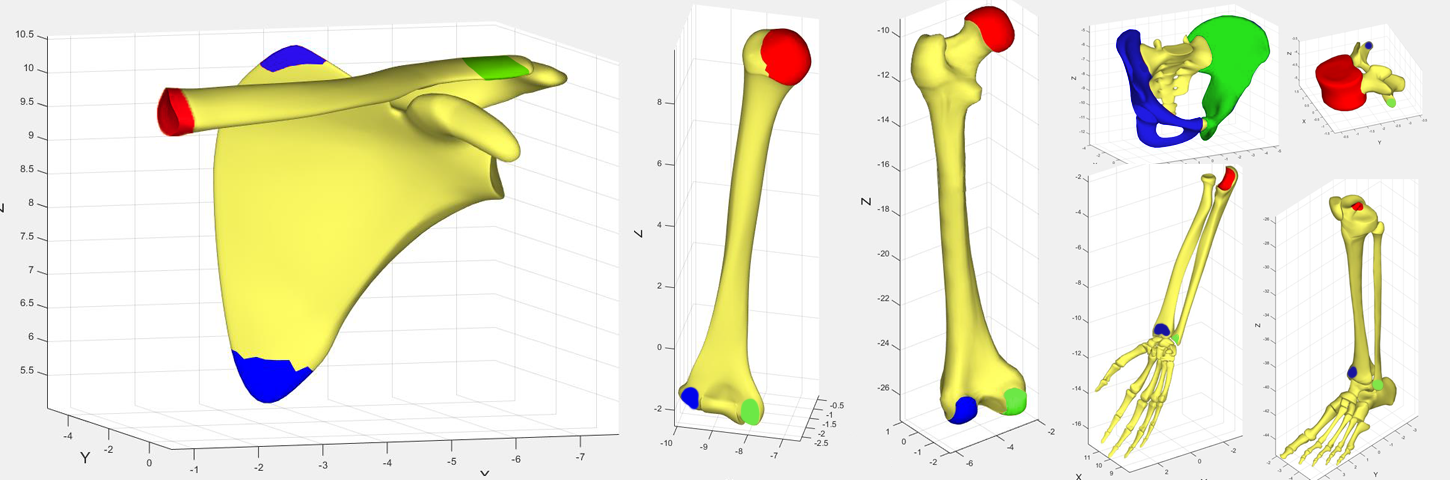
\includegraphics[width=0.95\textwidth]{IMG/rigshoulder.png}%[width=0.8\textwidth]
    \caption{La imagen muestra los huesos del modelo de referencia antes de registrar los datos del paciente. Las áreas coloreadas se utilizan para calcular el sistema de referencia de cada articulación. El centro de rotación se calcula a partir de las zonas rojas. Dos vectores ortogonales se calculan con las zonas azul y verde. El tercer vector ortogonal se calcula en base a los dos anteriores.}
\label{fig:humero}
\end{figure}


%%%%%%%%%%%%%%%%%%%%%%%%%%%%%%%%%%%%%%%%%%%%%%%%%%%%%%
\subsection{Volumetrización}
\label{posing:volumetrizacion}
%%%%%%%%%%%%%%%%%%%%%%%%%%%%%%%%%%%%%%%%%%%%%%%%%%%%%%
%
Como se ha introducido anteriormente, el objetivo es crear un campo de desplazamientos continuo que permita mover la anatomía interna del paciente virtual. El algoritmo discretiza el interior del modelo utilizando la piel y el tejido óseo como referencia, obteniendo una malla volumétrica formada por tetraedros. %\del{Esta malla de tetraedros es una pieza clave del algoritmo que se utilizará para calcular el citado campo de desplazamientos.}
La siguiente etapa (sec. \ref{posing:Pesado}) calculará la influencia del movimiento de cada hueso en los vértices de los tetraedros, de forma que el movimiento de los huesos afecte a los vértices de la malla volumétrica. El campo de desplazamientos se obtendrá de forma implícita interpolando el desplazamiento de los vértices en el interior de los tetraedros, mediante el uso de coordenadas baricéntricas. %\del{Esta malla será fundamental en las siguientes etapas.}
%\del{Después, esta malla será donde se calcule el campo de desplazamiento (Sec. \ref{posing:Poses}). También, el campo de desplazamientos guiará la animación del modelo virtual gracias al cálculo del mapeado entre los tetraedros generados en esta etapa y los distintos tejidos (Sec. \ref{posing:Mapeado}).}  \todo{Estas ultimas frases son muy raras, sobretodo la final. Explicas cosas que no son necesarias para esta etapa. }


%\todo{No te das cuenta de confusa que es esta frase. Lo que quieres decir es que no calculas directamente la malla de tetraedros, primero creas una imagen volumétrica. Reescribe}
%\del{En lugar de proceder al proceso de discretización con las representaciones superficiales de los tejidos, se ha optado \new{por} generar una representación volumétrica a partir de la piel y los huesos como paso intermedio para controlar el proceso de discretización y mejorar la robustez del algoritmo. Se genera una imagen en tres dimensiones compuesta por \emph{vóxeles}\footnote{unidad cúbica mínima para representaciones volumétricas} que permitirá simplificar el etiquetado aquellos \emph{vóxeles} que \del{colisionan con} \new{pertenezcan a} la piel y los huesos.}\todo{simplificar?}
La malla volumétrica no se calcula directamente a partir de la representación superficial de los tejidos del paciente. En su lugar, se construye una imagen tridimensional en la que se etiquetan los \emph{vóxeles}\footnote{unidad cúbica mínima para representaciones volumétricas} que pertenecen a los huesos y la piel del paciente virtual. Este paso intermedio permite controlar el proceso de discretización y mejora su robustez.
%\del{La malla volumétrica no se realiza de forma directa, sino que se ha decidido general una representación superficial a partir de la piel y los huesos como paso intermedio para controlar el proceso de discretización y mejorar la robustez del algoritmo. Se genera una imagen en tres dimensiones compuesta por \emph{vóxeles}}\del{  que permitirá simplificar el etiquetado aquellos que pertenezcan a la piel y los huesos. }
El tamaño de la imagen 3D depende de los tamaños del \emph{vóxel} y de la caja contenedora del modelo. Cuanto más grande sea dicha caja y el tamaño del \emph{vóxel} más pequeño, más detalle tendrá la imagen 3D resultante. Un elevado número de \emph{vóxeles} implicará un mayor consumo de tiempo y memoria.
%\del{Sin embargo, hay que tener en cuenta que a más detalle, más tiempo de cálculo y más consumo de memoria será necesario.}
%\todo{sigue sin gustarme la frase. Piensala más}
En esta tesis se ha establecido un tamaño de celda que permita tener como máximo una caja contenedora de tamaño 250x700x120 \emph{vóxeles}, en todos los modelos probados.

El proceso de \emph{voxelización} empieza etiquetando aquellos \emph{vóxeles} que coinciden con la piel (Fig. \ref{fig:voxelizacion}.a). Después, los \emph{vóxeles} interiores se etiquetan usando la técnica descrita en \cite{SUZUKI20031} (Fig. \ref{fig:voxelizacion}.b).
%\todo{expresalo de otra manera}
En este punto, se ha decidido añadir una etapa en la que se eliminan los \emph{vóxeles} marcados como piel (Fig. \ref{fig:voxelizacion}.c). %\del{donde aquellos \emph{vóxeles} que pertenecen a la superficie de la piel vuelven a estar no etiquetados \del{como vacíos}}. 
Este paso se ha introducido para mejorar la robustez del método en zonas que podrían quedar interconectadas por su proximidad. 
%\todo{No pongas resultados pon la referencia!}
En el apartado \ref{posing:result} se mostrará como esta etapa mejora el resultado final y evita problemas importantes. Finalmente, se procede a etiquetar los \emph{vóxeles} que corresponden a cada hueso como se muestra en la imagen (Fig. \ref{fig:voxelizacion}.d), de forma similar al procedimiento que se siguió con la piel. 
%
%\todo{puedes hacer la imagenes más grandes. No hay limite de espacio!}
%
\begin{figure}[th]
   \centering
    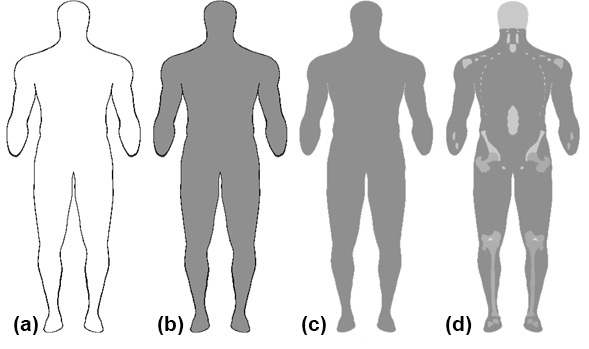
\includegraphics[width=0.95\textwidth]{IMG/Volume2.png}
    \caption{
    Cortes coronales de la imagen volumétrica en las distintas etapas del proceso de \emph{voxelización}.}
\label{fig:voxelizacion}
\end{figure}

%\todo{me gusta esta separación. Usala en el texto. Fase 1 voxelización, fase tetraedrización}
Una vez se ha construido la imagen 3D, se utiliza para crear una malla de tetraedros. Para la tetraedrización, se utiliza el algoritmo \new{de} \ac{RDT} \cite{jamin:hal-00796052}. Este algoritmo permite generar mallas de tetraedros multidominio a partir de mallas superficiales o imágenes 3D. A la hora de configurar el algoritmo, se debe alcanzar un compromiso entre precisión y eficiencia (ver anexo \ref{anexo:criterios}). En este caso, se ha configurado para incrementar los tetraedros alrededor de la piel y la superficie de los huesos. \new{En consecuencia,} De esta forma, se aumenta la resolución en aquellas zonas donde se requiere calcular la influencia de los huesos de forma precisa.
%permite obtener más detalle en zonas intermedias donde se resolverá la transición de pesos explicado en la siguiente sección.}
%\todo{Explica porque}

En este trabajo, se ha conseguido mantener el número de los tetraedros por debajo de $3.5\times 10^6$ y el número de vértices por debajo de $8 \times 10^5$. 
%\todo{Describe la figura }
\new{En la figura \ref{fig:tetra} se puede observar una tetraedrización del modelo \emph{ZygoteBody}$^{TM}$. Los tetraedros del interior del modelo se han coloreado de color morado, mostrando con un color diferente aquellos que pertenezcan a un hueso.}
%
\begin{figure}[th]
   \centering
    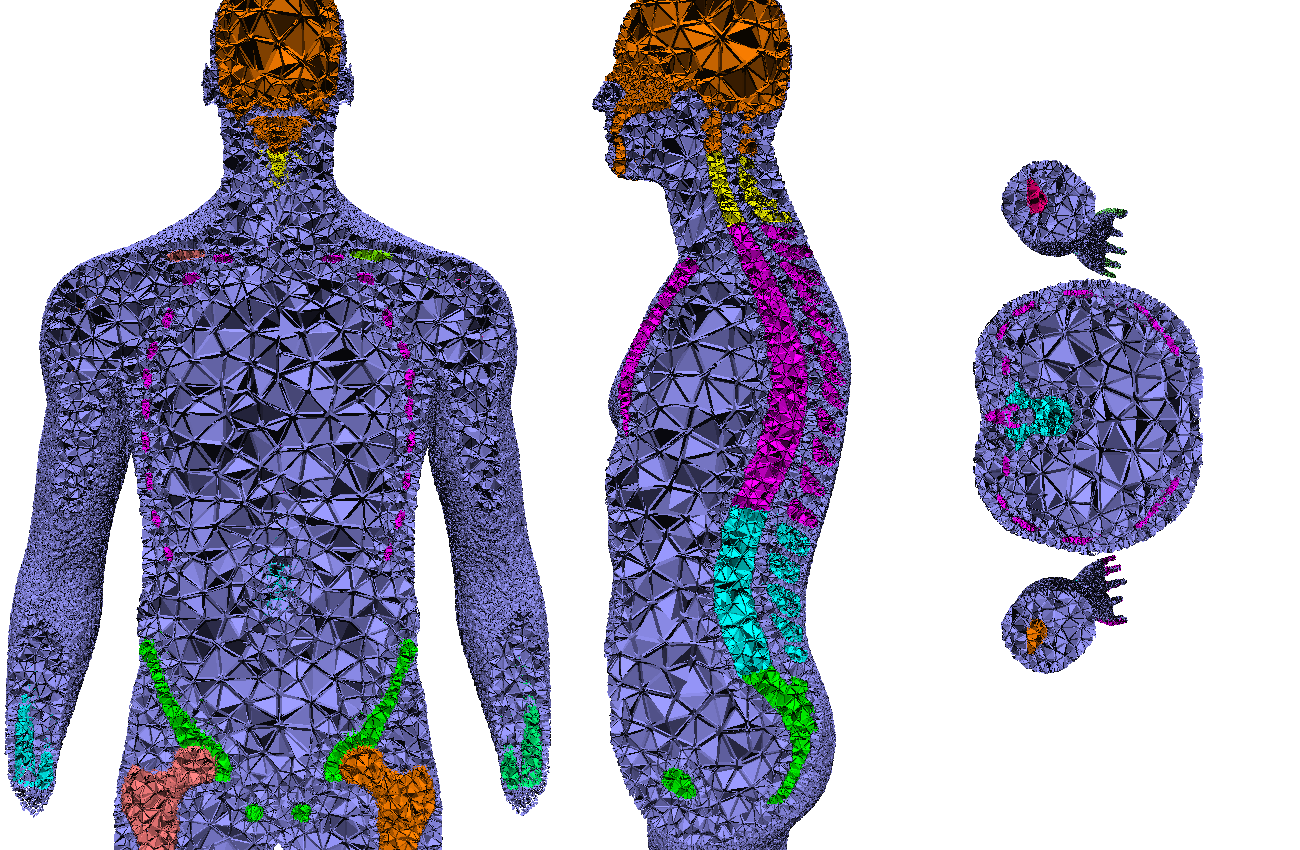
\includegraphics[width=0.95\textwidth]{IMG/boneid.png}
     \caption{Cortes coronales, sagitales y axiales mostrando el resultado de la tetraedrización. Los tetraedros morados representan el interior del modelo, mientras con diferentes colores se muestran los tetraedros etiquetados como hueso.}
\label{fig:tetra}
\end{figure} 
%\todo{Falta el color violeta}

%%%%%%%%%%%%%%%%%%%%%%%%%%%%%%%%%%%%%%%%%%%%%%%%%%%%%
\subsection{Pesado}
\label{posing:Pesado}
%%%%%%%%%%%%%%%%%%%%%%%%%%%%%%%%%%%%%%%%%%%%%%%%%%%%%%
%
Como se ha introducido en el estado del arte (ver sección \ref{art:pesado}), la etapa de pesado es donde se calcula como influye el movimiento de cada hueso sobre los vértices de la malla.
Tradicionalmente, esta etapa se realiza de forma manual por un artista ayudados por una herramienta  \ac{CAD}. Aun así, existen técnicas que pueden automatizar el proceso con ciertas restricciones. \emph{Baran y Popovi\'{c}} proponen en \cite{Baran:2007} una técnica de pesado automática donde se asume que el esqueleto virtual tiene forma de modelo de alambre y la malla superficial contiene completamente dicho esqueleto.
%\new{Es habitual encontrar que las técnicas citadas estan orientadas a utilizar mallas superficiales y utilizan una recta como representación del hueso virtual para calcular su influencia en los vértices.

Esta aproximación, no es directamente aplicable al algoritmo presentado, puesto que la mayor parte de la estructuras anatómicas del paciente virtual no contienen al tejido óseo. En esta tesis, se extiende el trabajo de \emph{Baran y Popovi\'{c}} de forma que puedan utilizarse mallas volumétricas en las que el tejido óseo esté etiquetado.  
%\del{Es habitual encontrar que las técnicas citadas están orientadas al pesado en mallas superficiales. Sin embargo, como se están tratando con mallas de tetraedros, hay que adaptar estos modelos a la problemática presente. }

%
%\todo{En el paso anterior no se calculó un campo de desplazamientos. Volumetrizó el espacio interior. El pesado calcula la influencia de los huesos sobre los vértices. Esta influencia se usa para mover los vértices siguiendo el movimiento de los huesos. Una ve que se han movido los vértices se calcula el campo de desplazamientos en el interior de cada tetraedro interpolando mediante coordenadas baricéntricas el desplazamiento de los vértices. En resumen la frase es confusa cambiala}.
%\del{A su vez, tampoco se desea calcular la influencia del esqueleto virtual, sino calcular como se propagan la influencia de los tejidos óseos sobre los demás vértices de la malla de tetraedros.}
%\todo{Piensa un poco más estas dos frases}
%\todo{No entiendo bien la idea}
%\del{Así pues, en este caso se va a calcular la influencia de los huesos reales y no de los huesos virtuales a los vértices de la malla de tetraedros y no de los vértices de los distintos tejidos}
%\todo{Separa las ideas. La primera diferencia es que no se usa el esquelto virtual, sino que se propaga la influencia del tejido oseo. Diferencia 2, no se calcula la influencia sobre el resto de tejidos sino que se calcuala la influencia sobre los vertices de la malla volumetrica}. 

%\todo{Esto es muy raro. Hablas de condiciones que no están en esta este capitulo. No se si se va enteder. Por favor, cuando lo reescribas dedicale tiempo.}

%Se ha tomado como punto de partida la técnica presentada en \cite{Baran:2007}. \emph{Baran y Popovi\'{c}} describen un proceso que realiza el pesado de forma automática, 
La técnica de pesado descrita en \cite{Baran:2007} asume que la influencia de los huesos varia suavemente en la superficie de la malla. Para ello, proponen utilizar la ecuación de la difusión \ref{diffusion}, suponiendo que la influencia de un hueso se propaga como lo haría la temperatura en una superficie. 

%\todo{Transiciones de que. Desarrolla un poco más las cosas}
%\todo{Tanto calor es un poco repetitivo.}

%Existen actualmente técnicas para calcular el pesado de forma más efectiva \cite{Jacobson:2011} comentadas en el estado del arte, pero se basan en el mismo principio\todo{que no se basen en el mismo principio no es suficiente para descartarlas}. 
%Tomando en cuenta la idea original de \emph{Baran y Popovi\'{c}}\cite{Baran:2007}, se ha modificado\todo{que se ha modificado} para adaptarla al algoritmo propuesto debido a que su aplicación no es directa\todo{reescribe la frase}.



%\todo{1. Rehaz la pasiba.}. 
%En \cite{Baran:2007}, se resuelve la ecuación del calor donde se hace una analogía entre temperatura y el peso de los vértices. 
%\todo{Cual es la analogía concreta. Ademas del la difusion del calor hablas en el parrafo anterior. Tienes que hilar mejor las cosas. }
\todo{Cuando metes una ecuación tienes que explicar los términos. }

\begin{equation}
\label{diffusion}
 \frac{\delta T}{ \delta t} = k \Delta T + q,
\end{equation}
%
donde $t$ es el tiempo, $T$ es la temperatura, $k$ es la conductividad térmica del material
y $q$ son los generadores de calor.
%\todo{revisar}

A la hora de calcular la influencia $Wj$ de cada hueso $j$, se resuelve la ecuación anterior en el caso estacionario: 
\begin{equation}
\label{diffusion1}
 0 =  \Delta W_j +  q_{k}.
\end{equation}
Ahora $q_{k}$ son las zonas de la malla superficial visibles desde el hueso $j$. Estos puntos son fuentes de influencia del hueso $k$. \emph{Baran y Popovi\'{c}} se ven obligados a introducir el término $q_{k}$ para relacionar los puntos de la superficie con el esqueleto virtual. 
%Dado que las condiciones de contorno se imponen directamente sobre la malla de tetraedros, no es necesario definir matrices de visibilidad que transfieran el calor desde los huesos virtuales a los vértices como ocurría en \cite{Baran:2007}. 
En el método propuesto en esta tesis, se dispone de una malla volumétrica del interior del paciente que se utiliza para calcular los pesos $W_j$:  
\begin{equation}
\label{diffusion2}
 0 =  \Delta W_j.
\end{equation}
La ecuación anterior se discretiza espacialmente mediante el \ac{FEM} utilizando nuestra malla volumétrica y las coordenadas baricéntricas de los tetraedros como función de forma (para más información puede consultarse el libro \cite{Lewis2004}):  

\begin{equation}
\label{diffusion3}
 0 =  \mathbf{A} \mathbf{W_j},
\end{equation}
donde $\mathbf{W_j}$ es el vector que contiene la influencia del hueso $j$ sobre todos los vértices de la malla y $\mathbf{A}$ es la matriz de coeficientes del sistema. 
Para poder resolver la ecuación \ref{diffusion3}, se deben establecer las condiciones de contorno del problema en los vértices etiquetados como hueso. De forma que la influencia $w_{i,k}$ del hueso $k$ sobre el vértice $i$ es igual a $1$ si $k=j$ e igual 0 si
$k \neq j$. Para introducir la condiciones de contorno se ha decidido utilizar la técnica de eliminación: 
\begin{equation}
\label{diffusion4}
 \mathbf{b_j} =  \mathbf{\hat{A}} \mathbf{W_j},
\end{equation}
donde la matriz $\mathbf{\hat{A}}$ se obtiene eliminando las filas y las columnas de los vértices que están etiquetados como hueso y  $\mathbf{b_j}$ es el vector de términos independientes que modela las condiciones de contorno del hueso $j$. Tal y como puede apreciarse en la ecuación \ref{diffusion4} la matriz $\mathbf{\hat{A}}$ es constante para todos los huesos, ya que solo depende de la discretización del dominio. Como esta matriz es simétrica y definida positiva, permite calcular la descomposición de \emph{Cholesky} una única vez y usarla para resolver el sistema lineal de cada hueso.





%\todo{No explicas los términos de la ecuación. antes de hablar de Wj yo hablaria de Wi,j. Por otro lado recuerda que los vectores debería ir en negrita. Deberías intidicar que resuelves la equación en el caso estacionario. Es uno de los motivos de que se simplifique. Cita el libro que uilizamos  }

%De esta forma, se obtiene un campo de pesos $W_j$  para cada hueso donde el tejido óseo correspondiente a $j$  propaga su influencia (temperatura 1) en el que se está resolviendo e influencia nula (temperatura 0) para el resto de huesos.  %de forma que la solución propuesta hace que la energía laplaciana sea estacionaria. Además, esta adaptación asegura una suavidad de orden superior\todo{la frase no suena bien}. 
%\todo{reescribe la frase. Da la sensación que no entiendes que escribes.: flojeo un poco en esta parte sobre todo al escribirla 1 Reformulamos el problemas haciendo cero el laplaciano. Esto es equivalente a minizar la energia. 
%Tienes que hacer un esfuerzo: 
%Ver enlace en comentarios
%https://es.wikipedia.org/wiki/Operador_laplaciano 
%}
%


%Con el objetivo de calcular  de un hueso $j$, se resuelve el caso estacionario definido en la ecuación \ref{diffusion}.%\todo{Tengo la impresion de que sueltas frases sin preocuparte de que sigan un orden logico. Esto está muy flojo.}
%\todo{Lo hablamos en persona. No me gusta la notación}

%A continuación, para calcular los pesos $W_j$, esta ecuación se resuelve para cada hueso $j$, donde se imponen las siguientes condiciones de contorno: se considera que el valor $W_j$ es $1$ (influencia) dentro de los tetraedros etiquetados como $j$; y el valor es $W_j$ es $0$ (influencia 0) dentro de los tetraedros etiquetados como $k$, donde $k$ es cualquier otro hueso que no es $j$. En el equilibrio estático, el resto de vértices tienen que verificar la ecuación \ref{ourdiffusion}. El problema se define de la siguiente manera:

% \begin{equation}
% \label{problema1}
% \Delta W(x)_{j} = 0 \\
% \end{equation}
% \begin{equation}
% \label{problema2}
% W(x)_{j} = 1\ \;
% \forall x \in B_{j} \\
% \end{equation}
% \begin{equation}
% \label{problema3}
% W(x)_{j} = 0\ \;
% \forall x \in B_{k}; k\neq j
% \end{equation}
%\new{donde $W$ es el campo de pesos definido en el dominio $x$. $j$ indica el hueso para el que se está resolviendo, mientras que B es el subdominio de $x$ que representa el hueso real.}

%
%En comparación, a un mayor número de vértices perteneciente a la malla de tetraedros, el sistema de ecuaciones resulta mucho mayor.}
%\new{Con el objetivo de resolver la ecuación \ref{problema1}, se discretiza usando \ac{FEM}  (ver \cite{Lewis2004}). La ecuación \ref{system} muestra la discretización final de la ecuación de difusión:}
%
%\begin{equation}
%\label{system}
%\mathbf{A} \mathbf{W}_j = \mathbf{b}_j,
%\end{equation}
%
%donde $\mathbf{A}$ es la matriz de coeficientes del sistema, el vector $\mathbf{b}_j$ depende de las condiciones de contorno del hueso  $j$ y $\mathbf{W}_j$ es un vector que  contiene los pesos  $w_{i,j}$ para cada vértice sin etiquetar $i$. \new{$\mathbf{A}$ es constante para todos los huesos ya que solo depende de la discretización del dominio. Como esta matriz es simétrica y definida positiva, permite calcular la descomposición de \emph{Cholesky} de esta matriz una única vez y usarla para resolver el sistema lineal de cada hueso.}

Al igual que los algoritmos de pesado clásicos, se deben cumplir las mismas condiciones, \ref{cond1} y \ref{cond2}, que se citan en en la sección \ref{art:pesado}. %Es importante mencionar que esta formulación cumple con las restricciones que se imponen en \ref{cond1} y \ref{cond2}. 
Primero, se puede asegurar que el valor máximo y mínimo sólo se alcanzan en los huesos (influencia $0$ o $1$).
Segundo, se puede calcular la suma de todos los vectores de pesos de resolviendo el siguiente sistema:
\begin{eqnarray}
\sum^{n}_{j=1} \mathbf{\hat{A}} \mathbf{W_j} = \sum^{n}_{j=1} \mathbf{b_j} \\
\mathbf{\hat{A}} \sum^{n}_{j=1} \mathbf{W_j} = \sum^{n}_{j=1}\mathbf{b_j} \\
\mathbf{\hat{A}} \mathbf{W}=\mathbf{b},
\end{eqnarray}
donde $n$ es el número de huesos. Dado que los huesos distintos de $j$ no modifican el valor de ninguna posición del vector $\mathbf{b_j}$ se puede concluir que el vector $\mathbf{b}$ modela un escenario donde todos los huesos tienen un peso de $1$ y por tanto $\mathbf{W}$  tomará el valor $1$ en todas sus posiciones. 


%si se considera \ref{min1}  y  \ref{min2}, donde  $n$ es el número de huesos, el sistema \ref{min3} equivale a calcular los pesos donde todos los puntos del contorno tendrán un valor de $1$. Además, como el máximo y el mínimo valor es alcanzado solamente en el contorno, dará lugar a que el valor de la suma de los pesos $\mathbf{W}$ será $1$, probando la condición \ref{cond2}.
%\todo{Creo que mezclas cosas}


% \begin{equation}
% \label{min1}
% b = \sum^{n}_{j=0} b_{j} 
% \end{equation}
% \begin{equation}
% \label{min2}
% W = \sum^{n}_{j=0} W_{j} 
% \end{equation}
% \begin{equation}
% \label{min3}
% A W = b
% \end{equation}

En trabajos más actuales, \cite{Jacobson:2011}, se presentaba una técnica que mejoraba la propuesta de \cite{Baran:2007}, donde se permitía crear puntos de anclaje y cajas contenedoras para controlar la animación del modelo. 
%\todo{lo que has antes de la coma no esta bien enlazado con lo que hay después.}
El inconveniente principal es la complejidad añadida al tener que resolver un problema disperso y cuadrático para imponer las restricciones. Sin embargo, la solución propuesta en esta sección solo requiere resolver un sistema de ecuaciones lineales. 
 %Por otra parte,  mientras que la técnica


%\todo{comprueba la sintaxis, parece cherokee }
 \begin{figure}[h]
   \centering
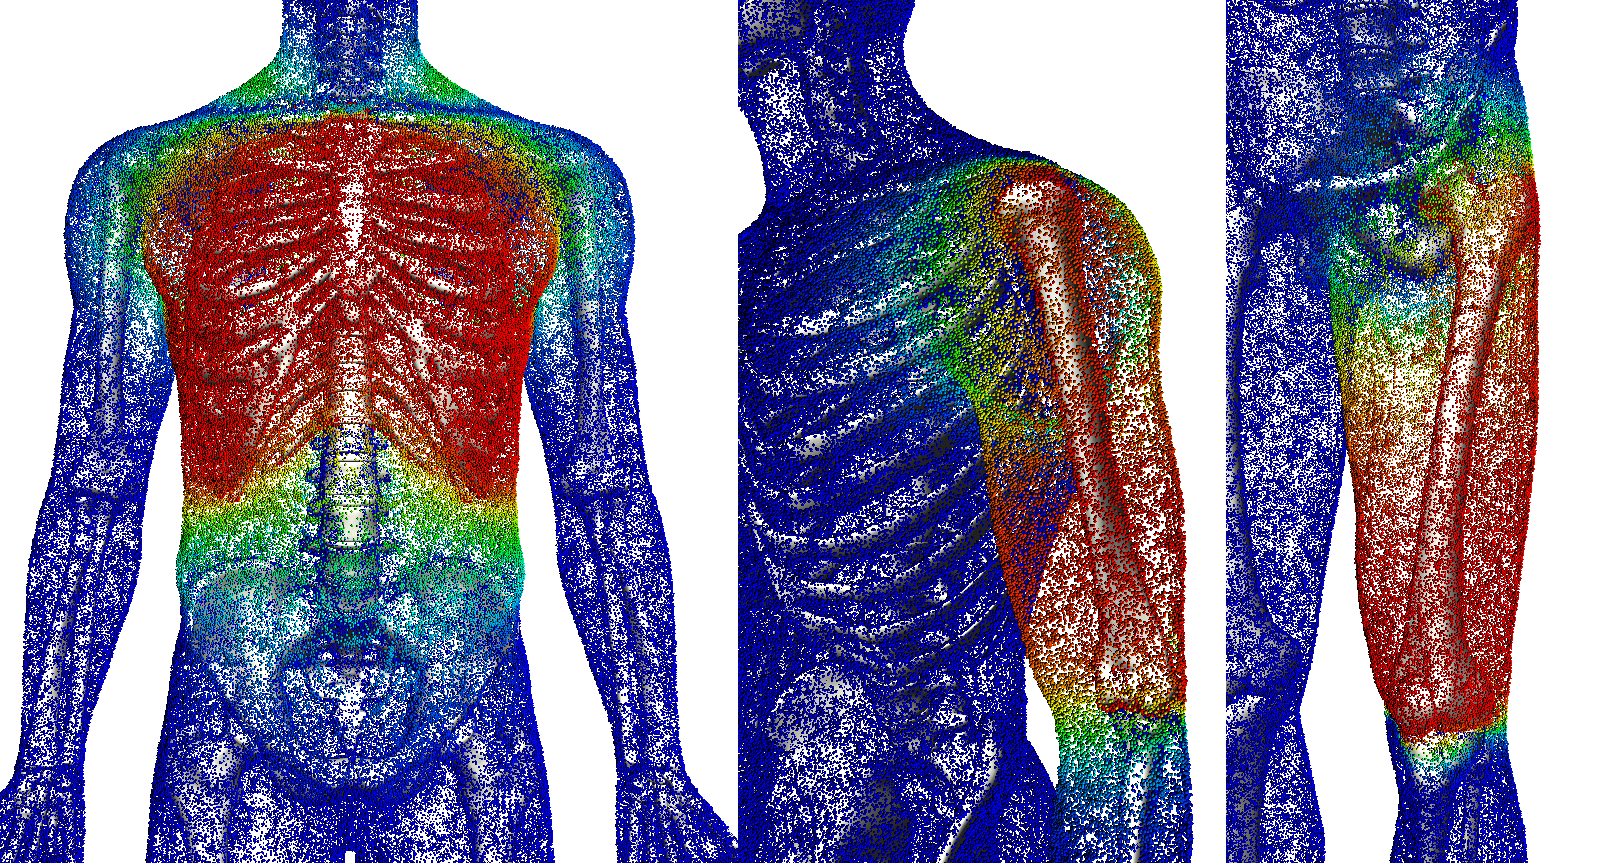
\includegraphics[width=0.9\textwidth]{IMG/weights.png}
     \caption{Influencia de algunos huesos sobre los vértices \del{de la} de la malla de tetraedros. En las zonas con color rojo\new{,} los pesos toman valores cercanos a 1 y en las zonas de color azul\new{,} los pesos son cercanos a 0.}
      \label{fig:pesado}
\end{figure}
 
En la figura \ref{fig:pesado} muestra los resultados obtenidos con el algoritmo propuesto. Se muestra  como ejemplo la influencia de los huesos de la caja torácica, el húmero y el fémur en los vértices de la malla de tetraedros.
%\todo{La idea esta bien pero la redacción es mejorable. Reescribe las dos frases.}

%%%%%%%%%%%%%%%%%%%%%%%%%%%%%%%%%%%%%%%%%%%%%%%%%%%
\subsection{Mapeado}
\label{posing:Mapeado}
%%%%%%%%%%%%%%%%%%%%%%%%%%%%%%%%%%%%%%%%%%
%
Para poder transferir los movimientos de las articulaciones a los tejidos del paciente, hace falta relacionar cada vértice de las mallas superficiales con las que se modela la anatomía con un tetraedro de la malla volumétrica. Para ello, es necesario conocer la posición del vértice en coordenadas del tetraedro en el que recaiga. \new{Y así, s}\del{S}e calculan sus coordenadas baricéntricas para \new{que}, de esta manera,  transferir el campo de desplazamientos definido en la malla de tetraedros\new{,} a los tejidos internos del paciente virtual.
%\todo{Esta frase no suena natural.}




%\new{Para calcular la influencia de los pesos de los teatraedros, se utiliza la posición del vértice que ocupa dentro de su tetraedro. Entonces, se utilizar ayuda de las coordenadas baricéntricas. }
%\todo{??????}
%
%Estas coordenadas indican la influencia de cada uno de los vértices del tetraedro al vértice que esta mapeado.
%Por tanto, hay que calcular cada una de las coordenadas baricéntricas para cada vértice de las mallas superficiales.
%\todo{De verdad que no puedo reescribir nada porque no se lo que quieres decir. Por favor rehaz todo el apartado con cuidado y ligando las ideas.}


Para encontrar el tetraedro que contiene a cada vértice de las mallas superficiales, el enfoque más simple es comprobar cada uno de los $n$ vértices con cada uno de los $m$ tetraedros. 
%
%\todo{La palabra significa suena raro en este contexto. La frase enter es rarr}
\new{Pero lamentablemente, este} \del{Este} método es muy costoso ($\mathcal{O}(n \cdot m)$). Para acelerar el cálculo global, se ha utilizado la técnica \emph{Spatial Hashing}\cite{Teschner2003}. Esta técnica subdivide el espacio en regiones cúbicas, almacenando en una \ac{tabla hash} solo aquellas regiones que contengan algún tetraedro. El coste de almacenar los tetraedros en la \ac{tabla hash} es $\mathcal{O}(m)$. Posteriormente, recorrer la lista de vértices de los distintos tejidos y asignarlos a un tetraedro tiene un coste lineal $\mathcal{O}(n)$, testeando solo los tetraedros que comparten posición en la \ac{tabla hash}. Dado que el proceso de volumetrización elimina la piel para evitar ciertos problemas, algunos vértices se encuentran fuera de la malla volumétrica. En estos casos, se busca de forma recursiva en la \ac{tabla hash}, el tetraedro más cercano.
\new{Y llegar de} \del{De} esta manera \new{a que se haya} \del{se ha} reducido el tiempo que tarda el método de fuerza bruta desde horas a menos de un minuto.


%\todo{No esta bien explicado}


%%%%%%%%%%%%%%%%%%%%%%%%%%%%%%%%%%%%%%%%%%%%%%%%%%%%%%
\subsection{Selección de poses}
\label{posing:Poses}
%%%%%%%%%%%%%%%%%%%%%%%%%%%%%%%%%%%%%%%%%%%%%%%%%%%%%%
%
Otro de los objetivos propuestos para este algoritmo es permitir a un médico \new{que} dirija y supervise la deformación del paciente virtual de manera interactiva. %A su vez, puede guardar posturas interesantes que permitan animar los modelos automáticamente en un futuro.
En esta etapa, el usuario es el encargado de seleccionar la postura del modelo anatómico. Para ello, el algoritmo propuesto permite usar cinemática directa, poses pregrabadas, animaciones, e incluso usar el dispositivo \emph{Microsoft Kinect}~\cite{shotton2013} para capturar la pose del usuario y transferirla al paciente virtual. Aun así, técnicas como \emph{retargeting} \cite{7581666} o cinemática inversa, podrían añadidase en el futuro. %ser incluidas en el algoritmo.
\todo{incluir imagen.}

En la animación esqueletal, para transferir el movimiento del esqueleto virtual a la malla superficial\new{,} se pueden utilizar diferentes algoritmos de \emph{skinning} (ver sec.\ref{art:skinning}). %\todo{el skinning no es un modelo matematico, son los algoritmos que transfieren el movimiento de los usos... Tal y como esta redacto parece que en el estado del arte has anticipado que TU ALGORITMO USARA EL SKINNING}.
%En el caso del algoritmo propuesto, se puede tratar los vértices de los tetraedros como vértices de una malla superficial\new{????}. De la misma manera que la animación clásica las animaciones esqueletales son transferidas a la malla volumétrica usando una técnica de \emph{skinning}. Los tetraedros deformados definen un campo de deformación que se utiliza para animar todos los tejidos del paciente virtual.
En el caso del algoritmo propuesto, las técnicas de  \emph{skinning} se aplicarán a los vértices de la malla de tetraedros en lugar de aplicarse directamente a las mallas superficiales. Los vértices del resto de tejidos del modelo serán transformados gracias al campo de desplazamientos definido en la malla volumétrica. Este se obtendrá de forma implícita interpolando el desplazamiento de los vértices de cada tetraedro en su interior\new{,} utilizando coordenadas baricéntricas para trasladar la deformación al paciente virtual. 

%\todo{A partir de ahora solo voy a dar pinceladas. Llevo la mañana del viernes, la del sabado y la del domingo y no avanzo. No puedo comentar cada frase. Es TU RESPONSABILIDAD cuidar la redacción. }


Se ha elegido implementar la técnica de \emph{skinning} descrita en \cite{le2016real},  ya que el método \ac{COR} resuelve algunos de los problemas de \ac{DQS} y \ac{LBS} descritos en la sección \ref{art:skinning}. El algoritmo se basa en calcular, en preproceso, los centros de rotación óptimos para todos los vértices de la malla. %En este caso, es necesario  de tetraedros\todo{paredce que son ellos trabajan con mallas de tetrahedros}. 
Una vez se calcula esta información, el rendimiento del algoritmo es muy similar al de otras técnicas como \ac{LBS} y \ac{DQS}. %Estas tres técnicas son intercambiables entre si debido a que están perfectamente diseñadas para usarse con las arquitecturas gráficas modernas.
Este algoritmo se basa en que los vértices con un pesado similar deben seguir las mismas transformaciones que sus vecinos. En su trabajo, \emph {Le y Hodgins} ~\cite{le2016real} proponen una función de similaridad  $s(\textbf{w}_p,\textbf{w}_s)$ con la que ponderar la contribución de los vecinos según lo parecidos que sean sus pesos:
%\todo{pasivas, intercambiables????}

%\begin{eqnarray}\nonumber
\begin{equation}
\label{similarity}
 s(\textbf{w}_p,\textbf{w}_s) = 
\sum_{\forall i \neq j} w_{p,i}w_{p,j}w_{s,i}w_{s,j}\exp-\frac{(w_{p,i}w_{s,j}-w_{s,i}w_{p,j})^2}{\sigma^2}
\end{equation}
%\end{eqnarray}
\normalsize
%
donde $\textbf{w}_p$ y $\textbf{w}_s$ son vectores de los pesos de los vértices $p$ y $s$, y se realiza la suma para todas las combinaciones de pares de huesos $i$ y $j$ . Por último, $\sigma$ parametriza la función exponencial. 
%\todo{faltan parámetros}
En el estudio que aquí se presenta se ha utilizado un valor de  $\sigma$ des $0.1$. 

La función de similaridad se utiliza posteriormente para calcular el centro de rotación $\textbf{cor}_p$ de cada vértice $p$. En \new{la presente} \del{esta} tesis, se ha adaptado la ecuación  propuesta en \cite{le2016real} de forma que pueda utilizarse en mallas volumétricas. Así la ecuación se quedará de la siguiente manera: 
%
\begin{equation}
%\begin{eqnarray}\nonumber
\textbf{cor}_p = 
\frac
  {
  \sum_{\forall t \in T}
    s(\textbf{w}_p,
      \frac{\textbf{w}_{t1}+\textbf{w}_{t2}+\textbf{w}_{t3}+\textbf{w}_{t4}}{4})
    %\frac{\textbf{v}_{t1}+\textbf{v}_{t2}+\textbf{v}_{t3}+\textbf{v}_{t4}}{4}
    V_t\mathbf{c}_t
  }
  {
  \sum_{\forall t \in T}
    s(\textbf{w}_p,
      \frac{\textbf{w}_{t1}+\textbf{w}_{t2}+\textbf{w}_{t3}+\textbf{w}_{t4}}{4})
    V_t
  } ,
%\end{eqnarray}
\normalsize
\end{equation}
%
donde $\textbf{cor}_p$ es el nuevo centro de rotación del vértice $p$, $t$ es el tetraedro de la malla de tetraedros $T$, $V_t$ es el volumen del tetraedro $t$, $\textbf{c}_t$ es el centroide del tetraedro $t$ y $\textbf{w}_{t1}$, $\textbf{w}_{t2}$, $\textbf{w}_{t3}$ y $\textbf{w}_{t4}$ son los pesos de los vértices del tetraedro $t$. Una vez calculado este centro, se puede usar en la etapa interactiva utilizando el \emph{shader} descrito en \cite{le2016real}.

Finalmente, para animar los vértices de cada malla, el campo de desplazamiento de un punto dentro de un tetraedro se puede calcular interpolando el desplazamiento de cada uno de sus vértices. Se interpola este campo usando las coordenadas baricéntricas de cada tetraedro, ya calculadas en el paso de pesado (sec. \ref{posing:Pesado}). Matemáticamente, el campo de desplazamientos calculado es continuo pero no diferenciable dentro de la malla volumétrica y permite calcular una matriz de transformación constante por cada tetraedro (consultar \cite{Muller2004}). Esta matriz de transformación, perteneciente al tetraedro, se aplica a cada uno de los vértices de la malla superficial asociados al tetraedro. Estos cálculos se realizan en la tarjeta gráfica para mejorar el rendimiento del algoritmo.

%\todo{No se si este apartado se entiende lo basta bien. Es muy criptioco. Redactado, a ver que tal}


% %%%%%%%%%%%%%%%%%%%%%%%%%%%%%%%%%%%%%%%%%%%%%%%%%%%%%%
 \subsection{Optimización}
\label{posing:optimizacion}
% %%%%%%%%%%%%%%%%%%%%%%%%%%%%%%%%%%%%%%%%%%%%%%%%%%%%%%
% %

% %

%Los resultados de la etapa previa son visualmente realistas\todo{¿Como lo sabes?}. \ac{COR} reduce el volumen ganado por \ac{DQS} o el volumen perdido por \ac{LBS}\todo{tienes resultados que lo respalden}. Aun así, hay algunos escenarios dónde se produce un cambio apreciable de volumen.El algoritmo propuesto permite al usuario refinar la solución usando un algoritmo basado en físicas
La mayoría de los cauces de animación se basan en transferir el movimiento de un esqueleto virtual a una \acl{B-rep} del personaje mediante un algoritmo de \emph{skinning}. Estos, suelen presentar el problema de garantizar la conservación del volumen. Las pérdidas y ganancias de volumen son comportamientos no deseados, especialmente, teniendo en cuenta que el cuerpo humano está compuesto principalmente por agua, un líquido incompresible. Por este motivo, se ha implementado un paso opcional que optimiza el resultado obtenido en la fase de \emph{skinning}. Esta técnica está basada en la formulación co-rotacional del \ac{FEM}. Cabe destacar que el objetivo de este paso es mejorar la conservación de volumen y no el de simular biomecánicamente el comportamiento de los distintos tejidos. Por este motivo, no se requiere de la caracterización de mecánica de paciente virtual.  

%Aunque se haya decidido utilizar un enfoque geométrico para el algoritmo, adicionalmente, se ha propuesto utilizar un modelo basado en físicas que permita al usuario refinar el resultado obtenido. Sin las descripciones mecánicas de los tejidos, se ha propuesto una solución que busca la conservación del volumen de cada tetraedro. Al no disponer de todos los tejidos o de las propiedades mecánicas, el objetivo de esta etapa no es conseguir un solución realista sino, mejorar el aspecto visual del resultado. }

%se puede decir que todos los tejidos están compuestos de agua y se asume que es un fluido incompresible y por tanto, las deformaciones tienen que permitir la conservación de volumen para cada tetraedro.}


%\todo{ponemos fórmulas que tenías en los comentarios?}
%\todo{Si eres capaz de explicarlo...}

El modelo físico utilizado está basado en un modelo mecánico estacionario:
\begin{eqnarray}
\nabla \cdot \mathbf{\sigma} = 0,
\end{eqnarray}
donde $\mathbf{\sigma}$ es el tensor tensión. También\new{,} se emplea un modelo elástico isotrópico, homogéneo y lineal:  
\begin{eqnarray}
\mathbf{\sigma} = \mathbf{E}\mathbf{\epsilon}, 
\end{eqnarray}
donde $\mathbf{E}$ es la matriz que define el comportamiento elástico del material y $\mathbf{\epsilon}$ es el tensor de \emph{Cauchy}. Es importante destacar que el tensor de \emph{Cauchy} no está indicado para medir grandes deformaciones.  Debido a su naturaleza lineal, las rotaciones generan distorsiones en la geometría al interpretarlas como deformaciones, produciendo efectos de escalado o abultamientos. Para resolver esta problemática, se utilizará la formulación co-rotacional del \ac{FEM} para resolver el sistema. La volumetrización del modelo (sec. \ref{posing:volumetrizacion}) se utiliza como discretización espacial y las posiciones de los huesos como las condiciones de contorno necesarias para resolver el problema estático. Para más información se puede consular \cite{Muller2004}.

Con la intención de controlar el modelo elástico planteado, se utilizan los parámetros \emph{ratio de Poisson} y \emph {módulo de Young}. El \emph{ratio de Poisson} controla la conservación del volumen, donde un valor del $0.5$ garantiza su conservación. Sin embargo,  se utiliza un valor ligeramente inferior para asegurar la estabilidad numérica. 
Por otro lado, el comportamiento elástico del material se caracteriza con el valor del \emph {módulo de Young}. Se va a utilizar un material homogéneo, ya que el valor de este parámetro es irrelevante desde el punto de vista teórico y, por tanto, se elegirá su valor con el objetivo de mejorar la estabilidad numérica del sistema. 
Para ello\new{,} se ha analizado la matriz de coeficientes del sistema para varios valores del módulo y se ha seleccionado aquel valor que haya maximizado su condicionante.

La formulación co-rotacional calcula las fuerzas internas (aquellas derivadas de la deformación)\new{,} tras deshacer las rotaciones de cada elemento de la malla. Después, rotará las fuerzas para ajustarlas a la configuración final del elemento~\cite{Muller2004}. Dado que esta técnica necesita conocer la rotaciones finales que se aplican a cada elemento de la malla, el problema estático se ha de resolver de forma iterativa. Para acelerar la convergencia del algoritmo, se utiliza la deformación seleccionada por el usuario como situación inicial reduciendo  significativamente el número de iteraciones requeridas para llegar a la solución final.  %(ver Fig. \ref{x}). 

Para conocer los desplazamientos de los vértices de la malla de tetraedros se ha formulado un sistema de ecuaciones lineales. Según las propiedades anteriormente citadas, la matriz de coeficientes del sistema lineal es dispersa, simétrica y definida positiva. Este tipo de sistemas de ecuaciones se pueden resolver utilizando el método del gradiente conjugado \cite{Press2007}. La convergencia de estos métodos se acelera con el uso de pre-condicionadores (ver \cite{hauth2003}). En el caso planteado, se utiliza un precondicionador de \emph{Jacobi} y, además, como solución inicial se utiliza la posición del modelo calculada en la etapa de \emph{skinning}. %Para acelerar esta etapa, se utiliza  como solución inicial la posición del modelo ya calculado en la etapa de selección de poses (sec. \ref{posingPoses}), además de emplear un precondicionador de Jacobi.

Finalmente, se utilizarán los desplazamientos de los vértices de los tetraedros para calcular la transformación que se aplicará a todos los tejidos asociados a cada elemento de la malla volumétrica, como se ha detallado en la sección \ref{posing:Poses}.% (ver sec. \ref{posing:Poses}). 

\subsection{Animación de representaciones volumétricas}
\label{posing:animvol}

\begin{figure*}[!ht]%[b]%[b!ht]
   \centering
   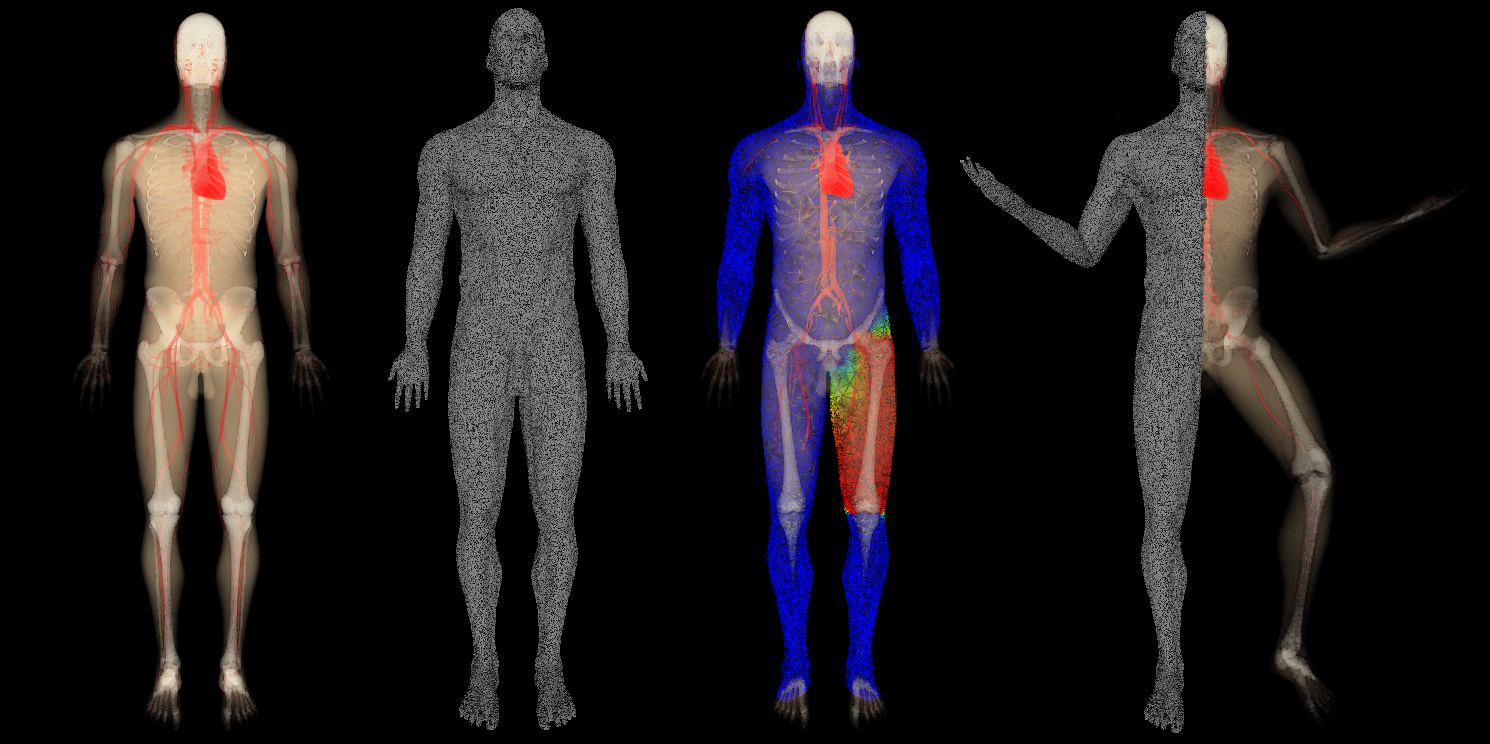
\includegraphics[width=0.90\textwidth]{IMG/Volumetric}
    \caption{Proceso de animación para modelo volumétrico. De izquierda a derecha: (1) modelo volumétrico en reposo, (2) malla de tetraedros generada, (3) malla de tetraedros representando el peso del fémur como ejemplo (rojo significa influencia cerca de 1, azul influencia 0) y (4) malla de tetraedros superpuesta al modelo volumétrico deformado. }
    \label{fig:volEx}
\end{figure*}
\todo{explica el por qué: el campo de desplazamientos, me he traido esto para inspirarme}

Como se puede leer en la sección 
\ref{posing:method}, el algoritmo se basa en el cálculo de un campo de desplazamientos continuo (ver sec. \ref{posing:volumetrizacion}) %\todo{si no es continuo todo lo que dices a continuación no sirve}
en el interior del paciente virtual que permita transformar sus estructuras internas. Esto permite deformar los tejidos de forma independiente y, aun así, garantizar que estos se muevan solidariamente. Se ha decido deformar los tetraedros y posteriormente interpolar el movimiento a los vértices usando las coordenadas baricéntricas, en lugar de transferir los pesos calculados (ver sec. \ref{posing:Pesado}) de los tetraedros a los vértices interiores. 
De esta forma, el campo de desplazamientos definido se puede usar para transformar tanto vértices de representaciones superficiales como \emph{vóxeles} en modelos volumétricos. 


\new{En la figura \ref{fig:volEx} se muestra los pasos para obtener una deformación de una representación volumétrica. En primer lugar, se genera la malla de tetraedros del modelo utilizando la misma técnica explicada en la sección \ref{posing:volumetrizacion}  y se calculan los pesos como se detalló en la sección \ref{posing:pesado}. A partir de esta \emph{tetraedrización}, se definen una serie de \emph{píxeles} dentro de cada tetraedro en la posición deformada. Se mapean con la configuración de reposo utilizando la transformación inversa del campo de desplazamiento. Para ello, se itera sobre cada caja contenedora de la \ac{tabla hash} y se utilizan las coordenadas baricéntricas. Este proceso, al ser fácilmente paralelizable en \ac{GPU}, permite que se pueda \emph{renderizar} en tiempo real.}



%%%%%%%%%%%%%%%%%%%%%%%%%%%%%%%%%%%%%%%%%%%%%%%%%%%%%%%%%
\section{Detalles de implementación}
\label{posing:preprocess}
%%%%%%%%%%%%%%%%%%%%%%%%%%%%%%%%%%%%%%%%%%%%%%%%%%%%%%%%%

Como se puede leer en la sección \ref{posing:req}, la selección de poses debe ser supervisada por un usuario y, por tanto, se debe permitir la animación del modelo de forma interactiva. 
Las etapas de \emph{rigging}, \emph{volumetrización}, \emph{pesado}, \emph{mapeado} y el \emph{cálculo de los centros de rotación} son las etapas más costosas computacionalmente. 
Por este motivo, dado que solo se tienen que ejecutar una vez por paciente virtual\new{,} se realizan en pre-proceso \new{y los} \del{. Los} resultados son guardados en ficheros adjuntos al modelo. 

Para facilitar la interacción, se ha creado una interfaz donde el usuario podrá manipular las articulaciones del paciente virtual\new{,} interactivamente y conseguir la transformación del modelo mientras es mostrado por la pantalla 

Por último, la etapa de \emph{optimización} no es posible que se ejecute interactivamente \del{. Esto depende del} \new{debido al} tamaño de la malla volumétrica resultante. Por ello, se deja a elección del usuario cuando se procede a ejecutar esta etapa.



\section{Resultados} 
\label{posing:result}
%%%%%%%%%%%%%%%%%%%%%%%%%%%%%%%%%%%%%%%%%%%%%%%%%%%%%%%%%
\todo{No me gustan los apartados. Separa entre rendimiento y calidad}

\todo{pasiva}
En esta sección se procede a mostrar como el algoritmo propuesto es usado para transformar distintos modelos virtuales de la posición de reposo que presentan, hasta la posición deseada. Dentro de estos modelos se incluyen modelos comerciales, otros procedentes de imágenes de pacientes reales o ejemplos diseñados para probar el sistema como se puede ver a continuación:\todo{qué se puede ver a continuación?}
\begin{itemize}
    \item \emph{ZygoteBody}$^{TM}$ Masculino
    \item \emph{ZygoteBody}$^{TM}$ Femenino
    \item \emph{Anatomium} Masculino
    \item \emph{Segmented Inner Organs}\cite{VoxelMan}
    \item Datos de pacientes reales
    \item Modelo de barra con cuatro huesos
\end{itemize}

\todo{lo dejo aquí. Reescribe todo}
Estos modelos han sido utilizados para ilustrar los resultados de probar las diferentes técnicas de \emph{skinning} utilizadas en esta tesis. 

\begin{figure*}[h]%[b]%[b!ht]
  \centering
  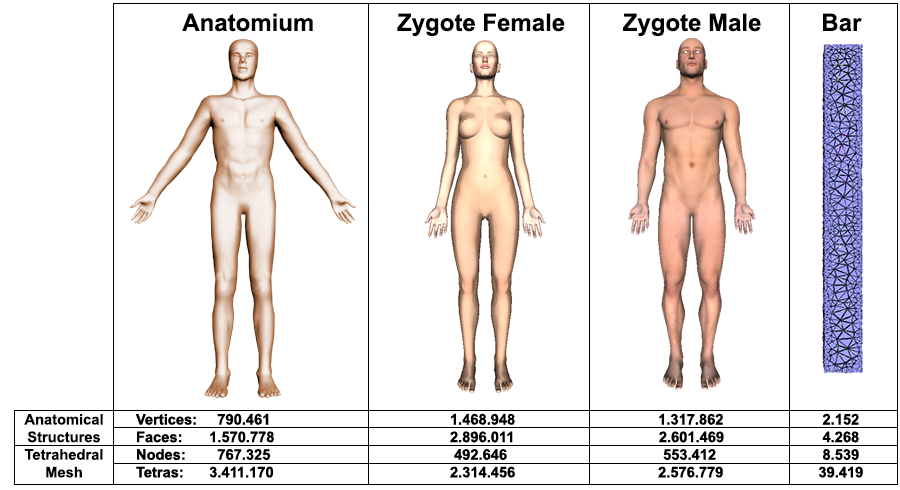
\includegraphics[width=0.90\textwidth]{IMG/models}
    \caption{Tamaño de los modelos usados en los test}
    \label{fig:models}
\end{figure*}

La figura ~\ref{fig:models} resume el tamaño de los modelos que se utilizarán y las mallas volumétricas asociadas a esos modelos. Es necesario remarcar las dimensiones de los modelos anatómicos y las representaciones volumétricas en comparación con los tamaños habituales vistos en la sección de estado del arte (ver sección \ref{art:animation}). En ocasiones, estos modelos tienen una complejidad de un orden de magnitud superior a las mostradas en la bibliografía.

Con el objetivo de no necesitar un usuario con habilidades artísticas o conocimientos avanzados de anatomía, se han utilizado animaciones procedentes de la base de datos de \ac{MoCap} de la \emph{Carnegie Mellon University}~\cite{CMUMCD}.

El computador utilizado para realizar todos los test de la presente tesis se compone de un procesador \emph{Intel\textregistered i7-4820K @ 3.7GHz}, tarjeta gráfica \emph{GeForce GTX 770} y 16GB de memoria \acs{RAM}.


\subsection{Proceso previo}
Como se ha descrito en la sección anterior, el algoritmo propuesto delega una serie de tareas a un proceso previo. Este proceso es realizado una vez por modelo y de las pruebas realizadas nunca ha excedido más de siete minutos. 


Hay que destacar que los modelos con los que se ha trabajado no están exentos de problemas. Por una parte, en ambos modelos de \emph{ZygoteBody}$^{TM}$ presentan auto-colisiones y se puede encontrar multitud de colisiones entre distintos tejidos. Además, zonas como la axila resultan zonas conflictivas como se puede observar en la figura \ref{fig:zygoteproblems}. 

Por otra parte, muchos de los procedimientos médicos se realizan en áreas localizadas, por lo tanto, muchas de las imágenes médicas disponibles no representan completamente el modelo anatómico del paciente. El algoritmo propuesto es capaz de tratar con información incompleta como podemos observar en la figura \ref{fig:patient} donde se muestra un modelo construido a partir de imágenes médicas reales.

\begin{figure}[h]
   \centering
    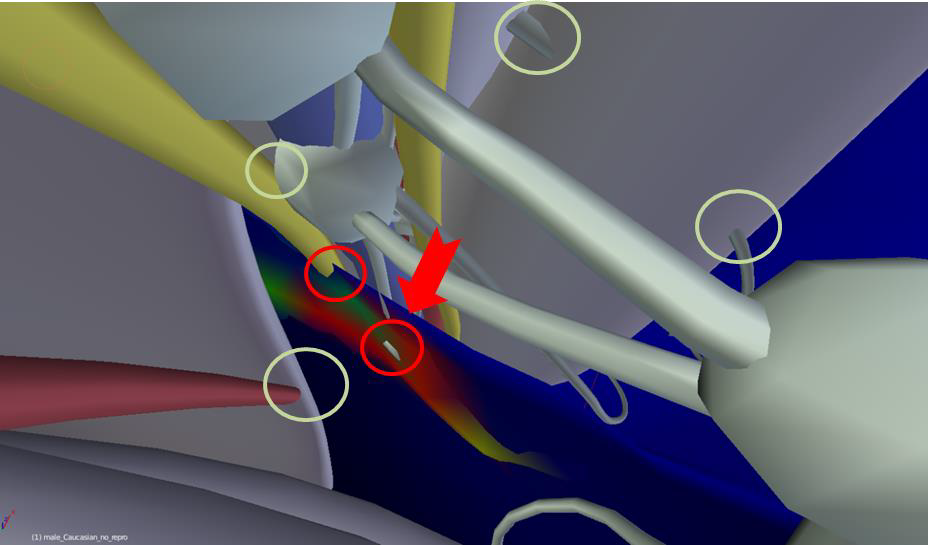
\includegraphics[width=0.5\textwidth]{IMG/zygoteproblems.png}
    \caption{Axila del modelo \emph{ZygoteBody}$^{TM}$ Masculino. Con círculos amarillos se observa colisiones entre diferentes tejidos. Los círculos rojos representan colisiones con el tejido de la piel  }
   \label{fig:zygoteproblems}
\end{figure}


%%%%%%%%%%%%%%%%%%%%%%%%%%%%%%%%%%%%%
\begin{figure}[h]
   \centering
    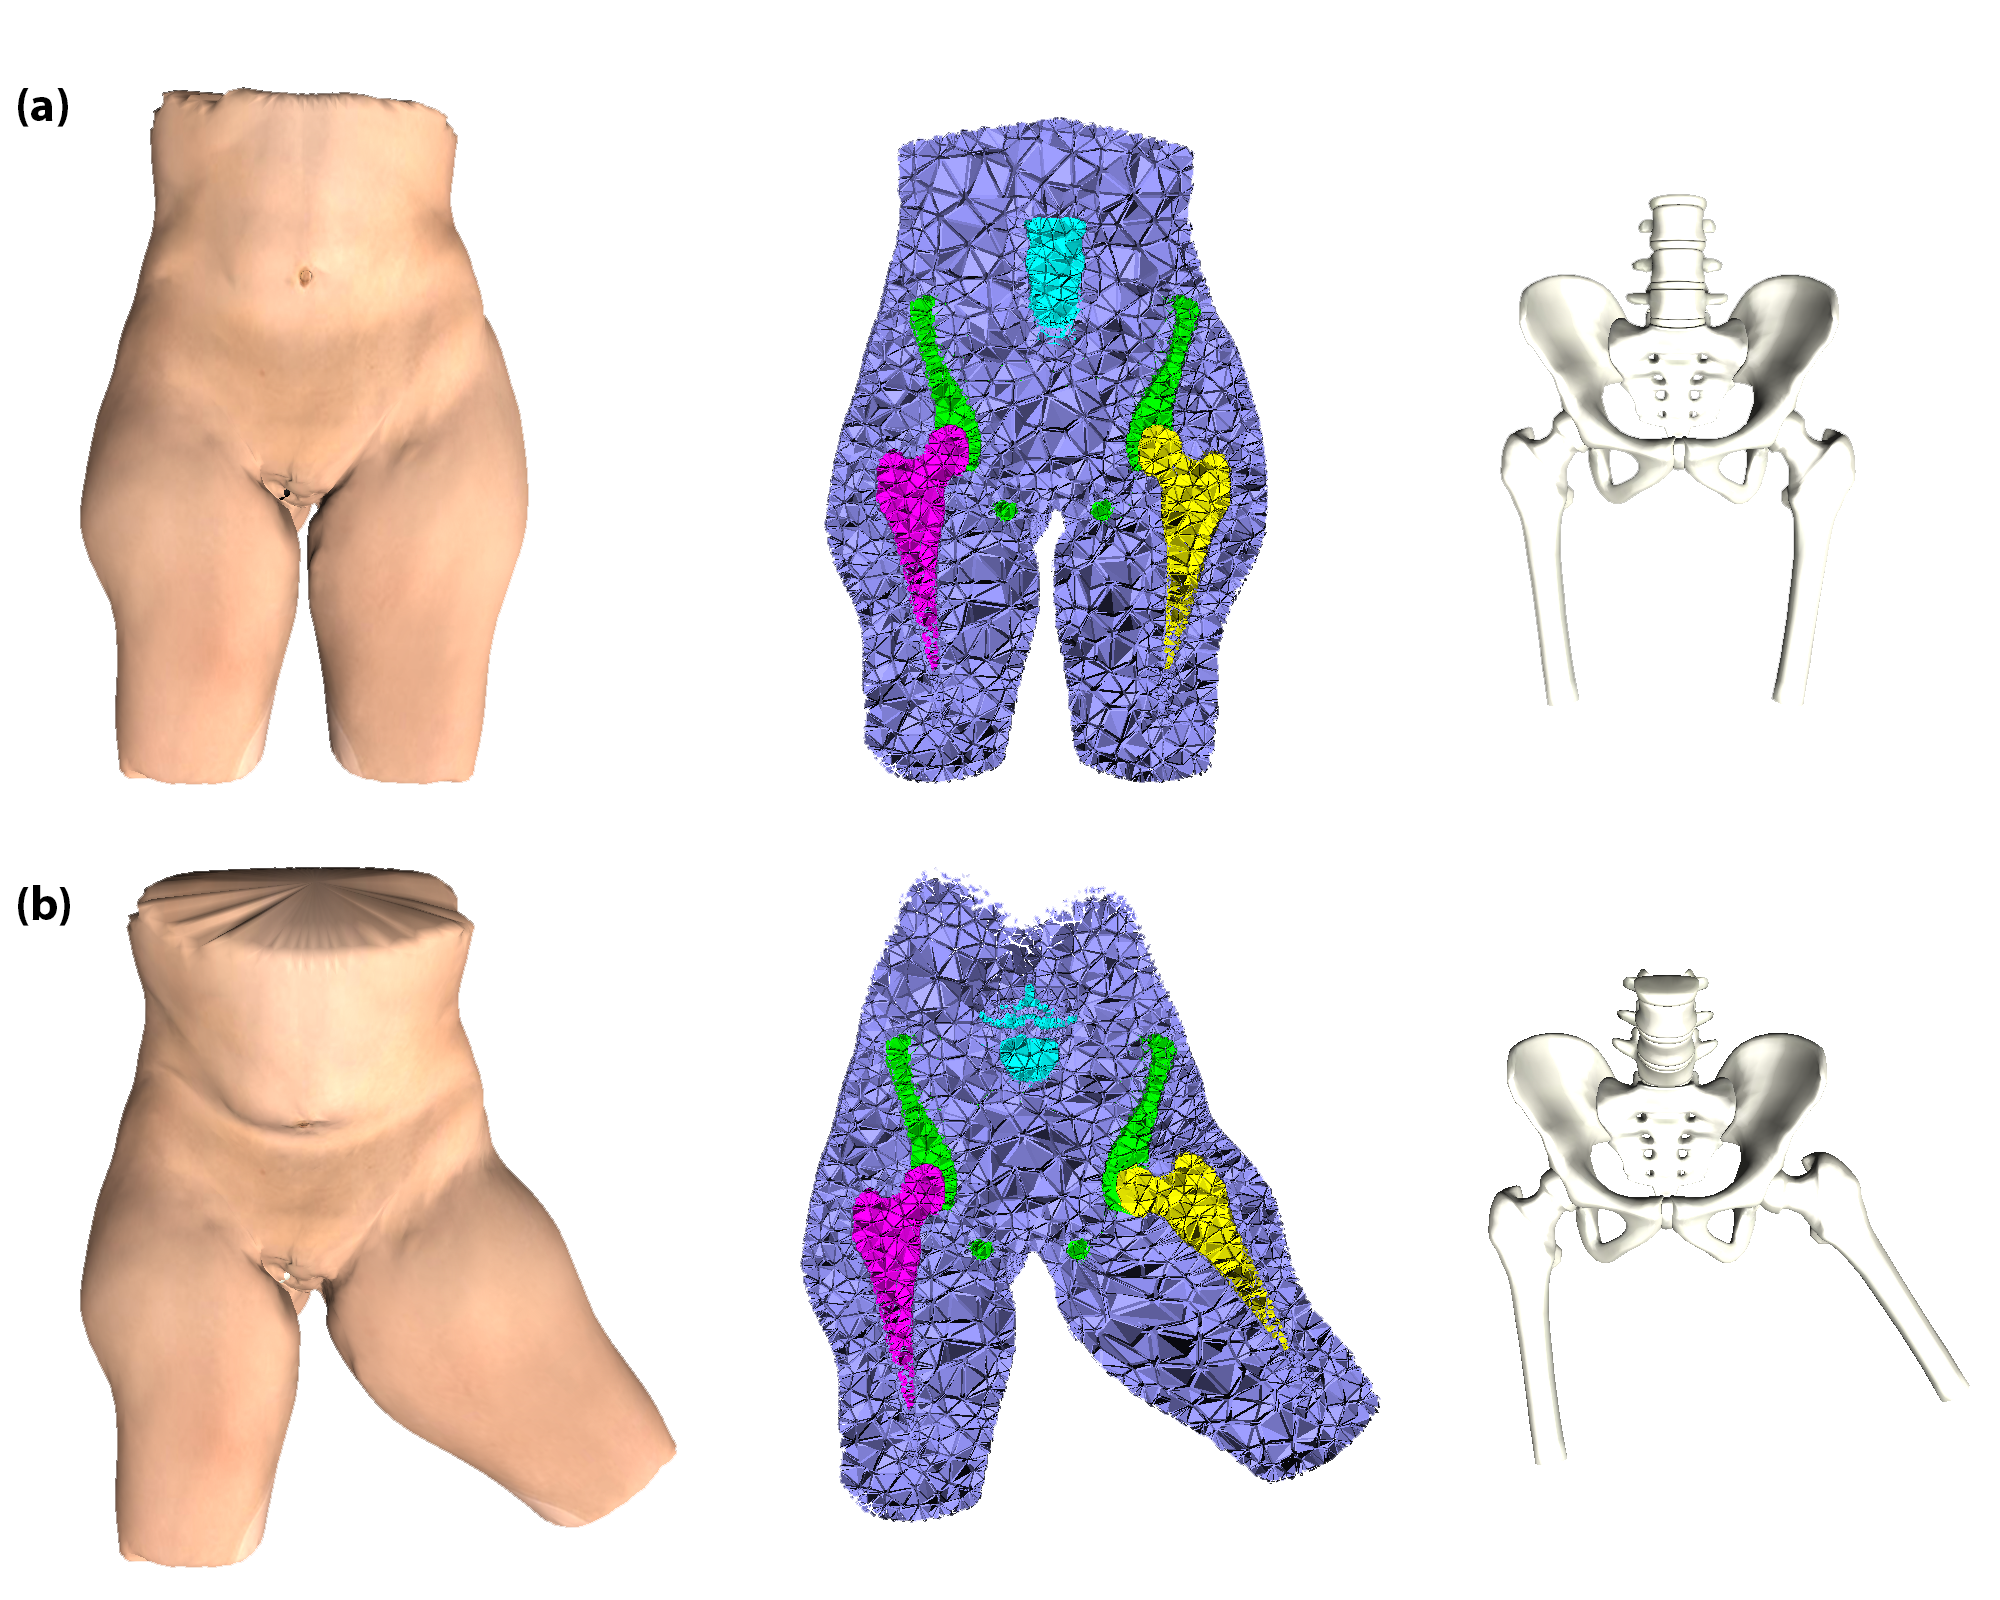
\includegraphics[width=0.5\textwidth]{IMG/patient.png}
    \caption{ La fila (a) muestra el paciente virtual construido a partir de datos de paciente real y se encuentran en posición de reposo. El algoritmo de posicionamiento permite modificar la pose de estos datos.
    }
   \label{fig:patient}
\end{figure}
%

Debido a la necesidad de que el algoritmo resulte robusto frente a los problemas comentados, se ha procedido a añadir diferentes ajustes en el algoritmo propuesto en varias de sus etapas.

En la etapa de \emph{volumetrización} (sec. \ref{posing:volumetrizacion}) se ha modificado la creación de la imagen volumétrica para borrar los \emph{vóxeles} etiquetados por el borde de la piel. Por tanto, en la figura \ref{fig:voxelizacion}.c se puede observar que los \emph{vóxeles} marcados como piel son desetiquetados con el objetivo de ser capaces de no crear tetraedros que conecten zonas del brazo y el pecho. En la figura \ref{fig:volsol} se puede observar la diferencia en la malla volumétrica. En la columna de la izquierda se muestra la \emph{voxelización} de la axila sin quitar los \emph{vóxeles} de la piel y en la columna de la derecha se puede observar que la zona de la axila esta correctamente.

\begin{figure}[h]
   \centering
    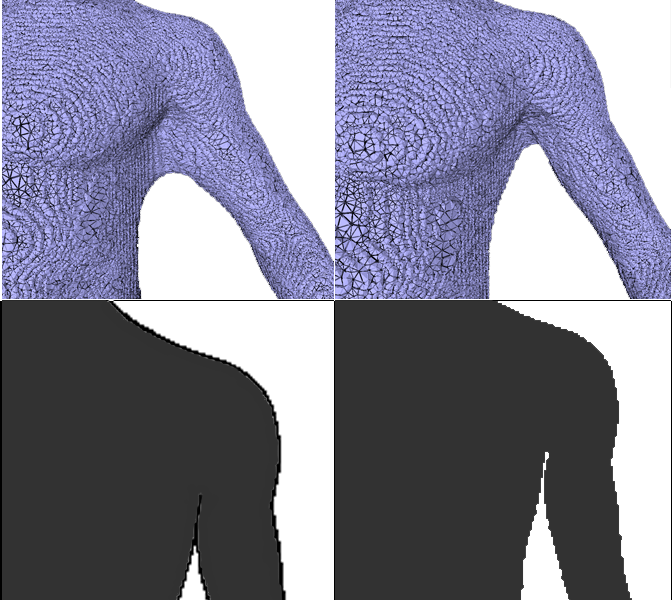
\includegraphics[width=0.45\textwidth]{IMG/volumetrizacion2.png}
    \caption{
    \emph{Volumetrización} de la zona de la axila. Columna izquierda muestra el problema de no eliminar los \emph{vóxeles} etiquetados como piel, en la columna de la derecha se resuelve el problema }
\label{fig:volsol}
\end{figure}


Con esta modificación se resuelve problemas de interconexión entre zonas no conectadas, aunque podría generar que se pueda encontrar tejidos que no están dentro de la malla volumétrica. Este problema sería adicional al que podría ocurrir donde el modelo que llega como entrada del \ac{TPTVPH} tuviera ciertos tejidos fuera de la piel. Debido a esto se ha propuesto una modificación de la etapa mapeado (ver sección \ref{posing:Mapeado}) para resolver este problema. Aprovechando la estructura espacial que proporciona la \ac{tabla hash}, aunque el vértice no esté dentro de ningún tetraedro, es fácil calcular el tetraedro más cercano para asociarle con él. Con esta modificación, en el caso concreto del modelo \emph{ZygoteBody}$^{TM}$ Masculino, alrededor de un 4.6\% de los vértices se encontrarían fuera de la malla volumétrica. 
Estos vértices no afectan de manera determinante en el proceso de mapeado. En este caso, el tiempo de mapeado es 36,35 segundos utilizando la \ac{tabla hash} como método de búsqueda. Este tiempo es muy pequeño si se compara con el tiempo que tardaría el proceso de mapear usando la técnica de fuerza bruta, que sería de 4 horas y 55 minutos para relacionar 1277325 de vértices a 2584115 de tetraedros en el caso del mismo ejemplo.  En la tabla \ref{tab:bruteforce} se muestra una comparación entre los tiempos empleados en mapear los distintos tejidos del \emph{ZygoteBody}$^{TM}$ Masculino con su malla volumétrica. Los modelos más complejos obtienen datos similares que se sitúan en torno a los cinco a siete minutos.


       
        
% \begin{landscape}
% \small
%  \centering % Center table
% \begin{center}
% \begin{tabular}{|c|c|c|c|c|c|  }
% \label{tab:forcebrute}

% \textbf{Modelo} & \textbf{Vértices} & \textbf{Vértices  huérfanos (\%)} & \textbf{Tetraedros (Elem./Vér.)} & \textbf{Spatial Hashing (ms)} & \textbf{Fuerza bruta (ms)} \\ 
% Skin                &32748      &89.81  &2,584,115 /555,702 &10678* &547967\\ 
% Muscles             &311600     &2.02   &2,584,115 /555,702 &12157* &4088365\\ 
% Nerves              &379008     &1.41   &2,584,115 /555,702 &12814* &5140770\\ 
% Connective Tissue   &168343     &0.68   &2,584,115 /555,702 &7881*  &2210942\\ 
% Lymphatic System    &5324       &5.66   &2,584,115 /555,702 &5456*  &702087\\ 
% Circulatory System  &380302     &4.29   &2,584,115 /555,702 &11541* &5008874\\ 
% TOTAL               &1277325    &4.6    &2,584,115 /555,702 &36.357103 &17.7*106 \\


% \end{tabular}.
% \caption{Brute force approach vs. spatial hashing approach.}
% \end{center}
% \normalsize
% \end{landscape} 




\todo{tabla enorme, como lo meto?}

Para finalizar de describir el proceso previo del algoritmo, a continuación se muestra la tabla \ref{tab:pre_pro} dónde se pueden consultar el tiempo empleado de cada etapa utilizando algunos de los modelos propuestos. 

\todo{meter todos los valores significativos de configuración}

Los valores de configuración para las distintas etapas son las siguientes:
La volumetrización no se hará en una caja contenedora más grande de tamaño 250x700x120. En cuanto a la función de similaridad empleada en la técnica de \emph{skinning} \ac{COR}, el valor de $\sigma$ que se utiliza es $0.1$.



\begin{table*}[!h]
\centering
\caption{Tiempo en milisegundos utilizado por cada etapa. ZM es Zygote Masculino, ZF es Zygote Femenino, A es Anatomium y CoR es la etapa de calcular los centros de rotación (sec. \ref{posing:Poses}).}
\begin{tabular}{cccccc}
\hline
\textbf{Modelo} & \textbf{Rigging} & \textbf{Volumetrización} & \textbf{Pesado} & \textbf{Mapeado} & \textbf{CoR }  \\ 
\hline
ZM  & 32698 & 69044 & 11762  & 51160   & 138005 \\ 
\hline
ZF  & 33251 & 63401 & 9171  & 71635   & 208886  \\ 
\hline
A   & 31891 & 120465 & 23318 & 44521  & 115214\\ 
\hline
\end{tabular}
\label{tab:pre_pro}
\end{table*}



\subsection{Selección de poses}

Con el objetivo que la selección de poses pueda ejecutarse en tiempo real, el proceso previo realiza las etapas más costosas computacionalmente que darán como resultado una serie de datos que serán usados por la herramienta al seleccionar el modelo virtual asociado. 

La etapa de selección de poses del algoritmo incluye la fase de \emph{skinning} para los vértices de los tetraedros y la consecuente deformación que es transferida a los tejidos del modelo virtual. Para mostrar de manera simple las diferencias visuales que se generan a través de las tres técnicas anteriormente citadas, se va a utilizar un modelo simple de un prisma rectangular con cuatro huesos virtuales en su interior. Este modelo por su simplicidad se utilizará para mostrar los resultados de rotaciones y giros para poder comparar entre técnicas utilizadas. En la figura \ref{fig:bar_bending} se pueden observar las diferencias visuales del método seleccionado (\ac{COR}) frente a los 2 métodos clásicos más conocidos en la literatura que son \ac{LBS} y \ac{DQS}. En cuanto a las rotaciones, se puede apreciar que en el caso de \ac{LBS} la articulación pierde volumen, sin embargo, en \ac{DQS} se puede observar un aumento de volumen. Respecto a los giros, es conocido que la técnica \ac{DQS} solventa el problema de \ac{LBS} donde la interpolación de los vértices se realiza de forma lineal produciendo el efecto \emph{candy-wrapper}. Así que, la técnica \ac{COR} es más robusta a cambios de volumen en rotaciones y además maneja adecuadamente los giros de las articulaciones. En esta figura se utilizan los tetraedros como referencia visual mostrando con los colores el pesado mostrado las diferentes influencias de los huesos virtuales. Se ha usado un código de colores, donde el color azul resultar ser los huesos impares que tienen influencia de 1 y el color rojo es donde los huesos pares tienen influencia de 1. Con este código de colores se puede observar las transiciones entre huesos.

\begin{figure*}[h]%[b]%[b!ht]
  \centering
  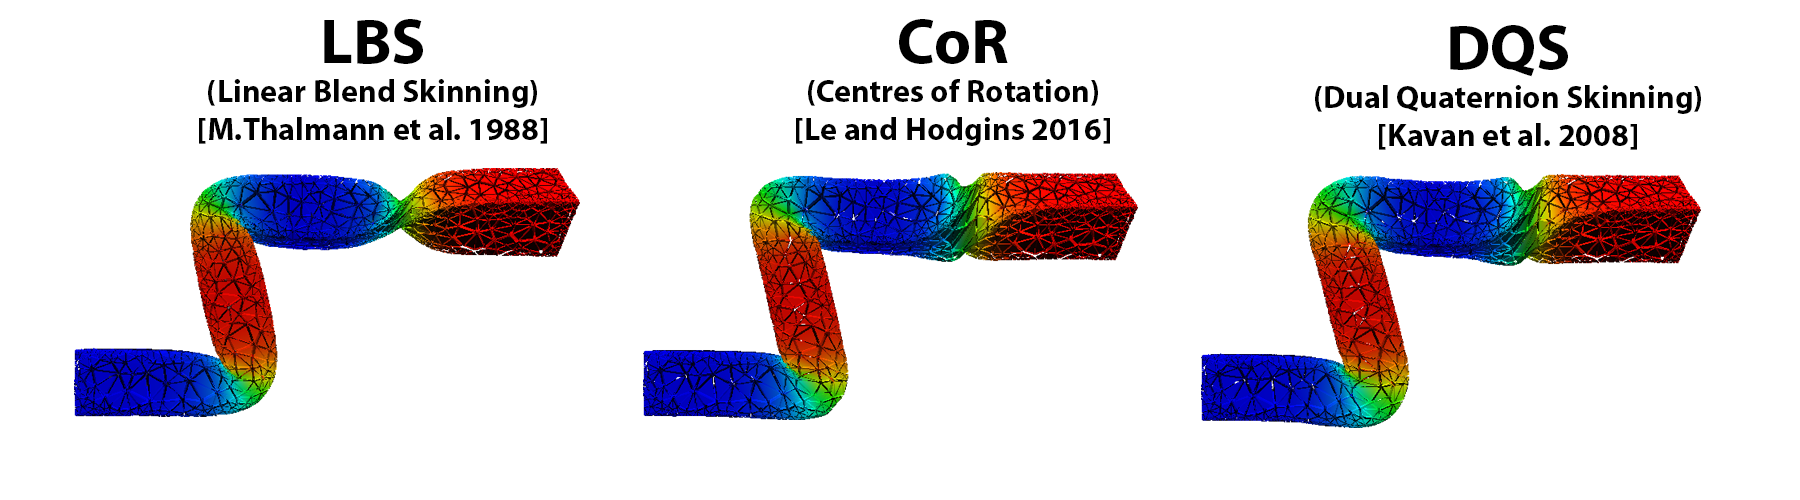
\includegraphics[width=0.90\textwidth]{IMG/BarraCoR}
    \caption{Deformación del prisma por las 3 técnicas. Primera rotación de 100º, segunda rotación de -100º y un giro de 135º.}
    \label{fig:bar_bending}
\end{figure*}
%%%%%%%%%%%%%%%%%%%%%%%%%%%%%%%%%%%%%

Una vez ilustradas las diferencias de manera teórica, a continuación se mostrarán las diferencias entre las distintas técnicas de \emph{skinning} utilizando los modelos anatómicos. En las siguientes figuras, se utilizará diferentes posturas de los modelos anatómicos para mostrar las diferencias en los resultados que producen cada uno de los métodos al deformar el paciente virtual.

En la figura \ref{fig:thigh_bending} se muestra una rotación de la articulación de la pierna. Las zonas perceptibles de producir artefactos son la zona superior del muslo en la zona inguinal y el glúteo. En esta imagen se puede observar que tanto la zona inguinal y el glúteo con la técnica \ac{LBS} produce una pérdida de volumen. En el caso de utilizar \ac{DQS} se aprecia el aumento de volumen predicho para esta técnica, sin embargo la técnica seleccionada \ac{COR} da como resultado un compromiso entre ambas técnicas. La imagen se acompaña con el tejido muscular en reposo como referencia y los tejidos circulatorio y nervioso de como el algoritmo propuesto es capaz de lidiar con toda aquella anatomía interna del modelo. En este ejemplo en concreto, las diferencias visuales entre técnicas de estos dos tejidos es mínimo al ser estructuras filiformes. 





% %%%%%%%%%%%%%%%%%%%%%%%%%%%%%%%%%%%%%
\begin{figure*}[h]%[b]%[b!ht]
  \centering
  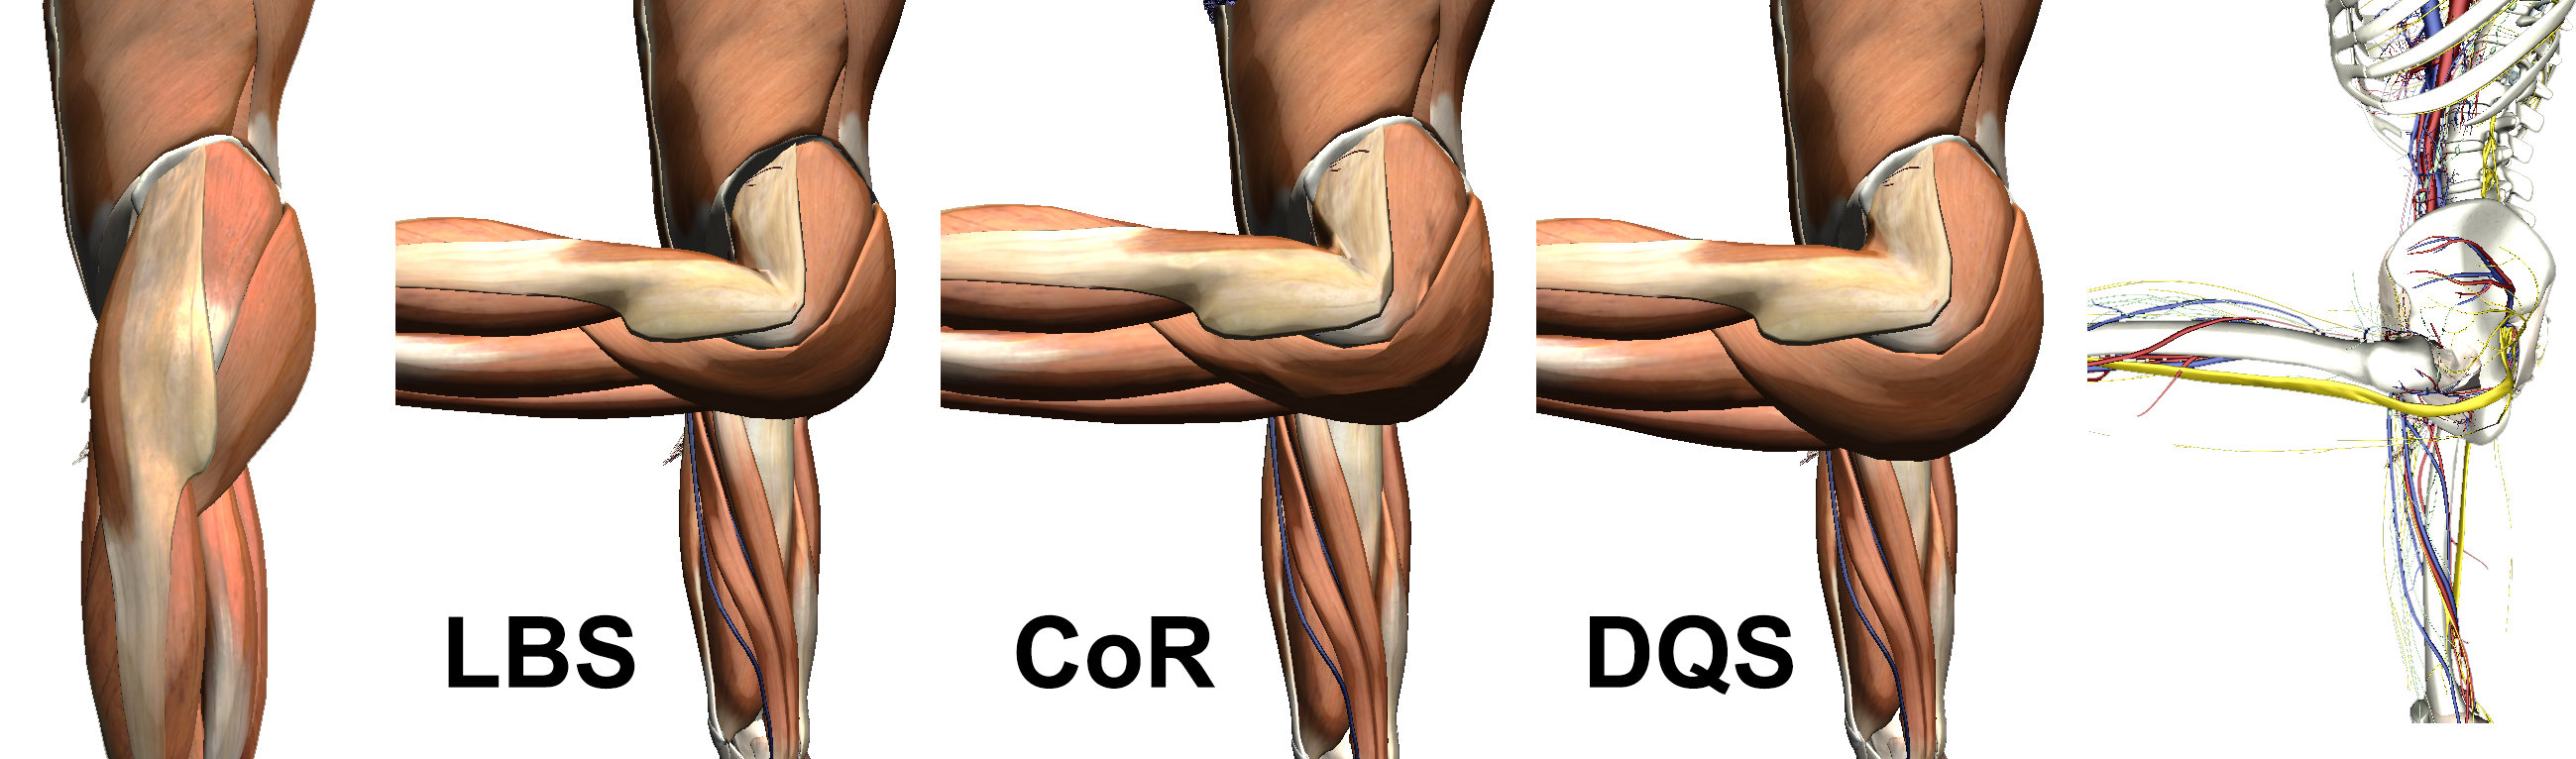
\includegraphics[width=0.90\textwidth]{IMG/compculo}
    \caption{ Deformación de una pierna. Izquierda: posiciones de los músculos en reposo; en el medio se muestran la pierna rotada usando las 3 técnicas de \emph{skinning} (\ac{LBS} pierde volumen tanto en el gluto como en la zona inguinal, \ac{DQS} añade volumen y \ac{COR} suaviza esos defectos; a la derecha podemos ver otros tejidos deformados.}
    \label{fig:thigh_bending}
\end{figure*}

\todo{más ejemplos aqui}
%%%%%%%%%%%%%%%%%%%%%%%%%%%%%%%%%%%%%

 Como se puede deducir de los requisitos descritos y la motivación de la presente tesis, se pretende que esta fase sea interactiva y el método debe ser capaz de manejar una gran cantidad de tetraedros (incluso con el gran tamaño de los ejemplos seleccionados). La tabla \ref{tab:inter} muestra el rendimiento  del método seleccionado (\ac{COR}) frente a los 2 métodos clásicos más conocidos en la literatura que son \ac{LBS} y \ac{DQS}. Como se puede observar, el rendimiento entre las diferentes técnicas son muy similares. La tabla muestra los valores máximos y mínimos de imágenes por segundo que es capaz de generar el algoritmo utilizando un ciclo de caminado para animar al modelo virtual.
%
\begin{table}[h]
\centering
\caption{Valores máximos y mínimos de imágenes por segundo durante el ciclo de caminado en la etapa de \emph{selección de poses} }
\begin{tabular}{cccc}
%\multirow{2}{*}{\textbf{Model}} & \multicolumn{2}{c}{\textbf{Interactive stage}} & \multirow{2}{*}{\textbf{Optimization}} \\
\textbf{Modelo}&\textbf{LBS} &\textbf{DQS} &\textbf{CoR} \\ 
\hline
ZM  & 111-90 & 100-90 & 100-76\\ 
\hline
ZF  & 76-60  & 66-52   & 60-50 \\ 
\hline
A   & 166-142 & 166-125 & 142-100\\ 
\hline
\end{tabular}
\label{tab:inter}
\end{table}


Con los resultados obtenidos, se puede afirmar que el algoritmo propuesto obtiene deformaciones visualmente realistas y es capaz de realizarlas en tiempo de ejecución delegando las etapas más pesadas a un proceso previo.

Finalmente, en la imagen \ref{fig:run1} se muestran resultados adicionales del uso del algoritmo con la técnica de \emph{skinning} \ac{COR} en los modelos \emph{ZygoteBody}$^{TM}$ Masculino y Femenino en diferentes situaciones.

%%%%%%%%%%%%%%%%%%%%%%%%%%%%%%%%%%%%%
\begin{figure*}%[h]%[b]%[b!ht]
   \centering
   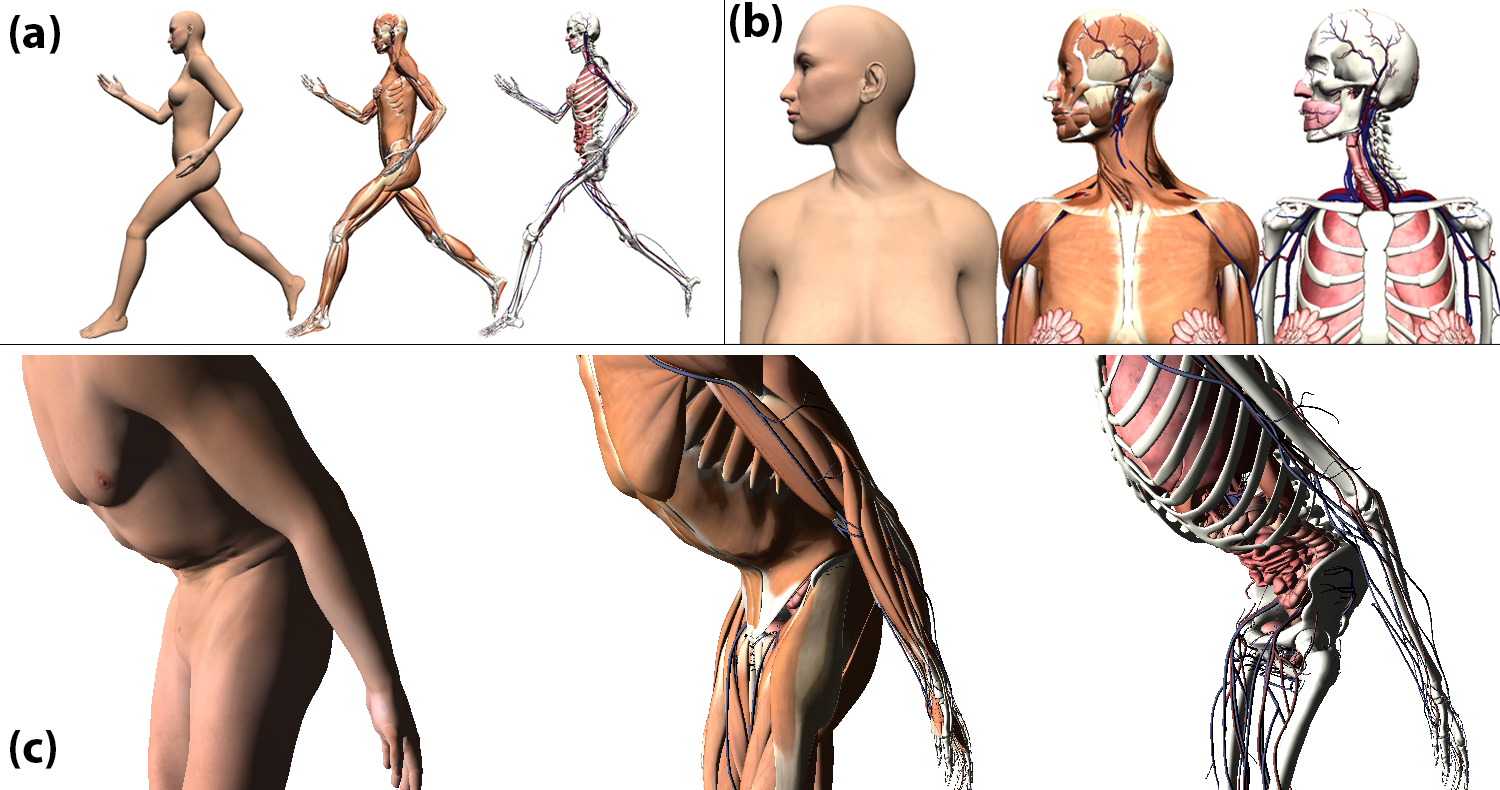
\includegraphics[width=0.90\textwidth]{IMG/examples}
    \caption{Resultados obtenidos utilizando \ac{COR}. (a): fotograma del ciclo de correr en el modelo ZF. (b): Cuello girado del modelo ZF. (c): Zona abdominal flexionada del modelo ZM.}
    \label{fig:run1}
\end{figure*}
%%%%%%%%%%%%%%%%%%%%%%%%%%%%%%%%%%%%%

\subsection{Optimización}

Las deformaciones resultantes de la etapa anterior dan como resultado poses visualmente realistas en la mayoría de los casos. La fase de \emph{skinning} basada en \ac{COR} solventa de forma efectiva los problemas típicos de las técnicas basadas en \ac{LBS} y de \ac{DQS}. Aún así, en algunas circunstancias se ha detectado un cambio no deseado de volumen. 
La técnica \ac{COR} no puede asegurar la conservación de volumen tal y como lo hacen las técnicas basadas en física. En esta sección, se va a comparar \ac{COR} con un modelo físico. Debido a que no se puede asegurar una apropiada descripción mecánica de los tejidos, el objetivo de esta optimización es garantizar la conservación del volumen.  Se ha propuesto utilizar la formulación \ac{FEM} co-rotacional para resolver el problema estático considerando un material lineal, isotrópico y homogéneo. En la mayor parte de los casos probados, con una iteración se obtenían resultados prácticamente indistinguibles de los resultados obtenidos con más iteraciones. 
 
%  Besides, the deformations are measured using the \emph{Cauchy} strain tensor. The boundary conditions, needed to solve the steady-state problem, are given by the positions of the vertices labelled as bones. The co-rotational formulation calculates the internal forces caused by the deformations in a non-rotated configuration. Then, the internal forces are rotated again into the final configuration \cite{Muller2004}. The algorithm needs to compute the element rotations in the final configuration. For this purpose, the solution is refined iteratively. The elastic used model can be tuned with two parameters: the \emph{Poisson ratio}  and the \emph {Young module}. The \emph{Poisson ratio} controls the volume conservation and it should take a value close to 0.5 (the real value has to be lower to ensure numeric stability). Since the material is homogenous, this value has no impact on the outcome. 
 Se ha escogido el módulo de \emph{Young}  intentado mejorar la estabilidad del sistema. Para ello, se han analizado distintas matrices de coeficientes del sistema, obtenidas a partir de distintos valores del módulo de \emph{Young}, quedándose con el valor que daba como resultado la matriz de coeficientes con menor número condicionante.
 
 La figura \ref{fig:anatomium} ilustra un ejemplo de cómo la técnica basada en la formulación \ac{FEM} soluciona alguna de los problemas de volumen que aparece con las otras técnicas. Sin embargo, debido a que la técnica \ac{COR} muestra buenos resultados se ha procedido a comprobar si esta optimización es elegida por los usuarios frente a la técnica geométrica.
 
 \begin{figure}[h]%[b]%[b!ht]
   \centering
   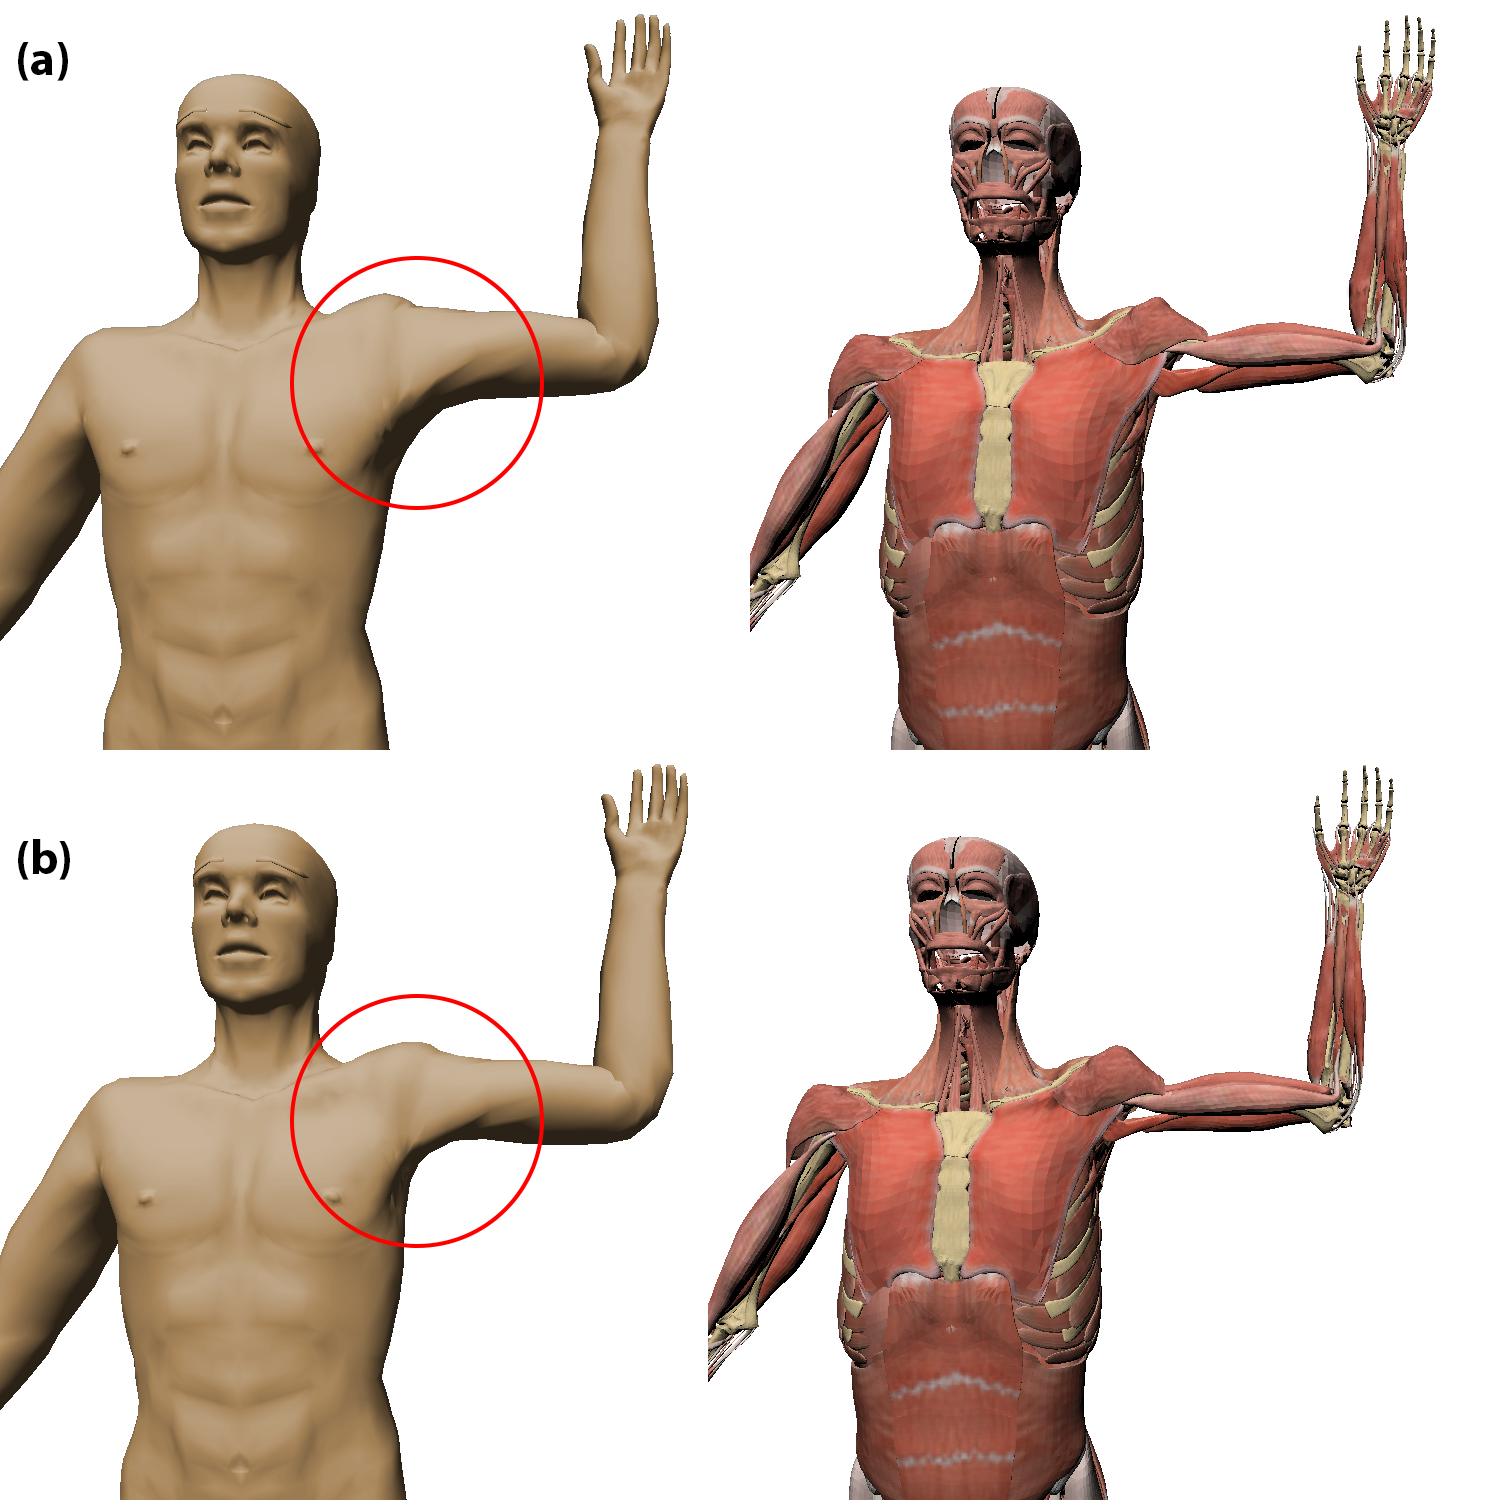
\includegraphics[width=0.45\textwidth]{IMG/AntCOR}
    \caption{ Comparación entre \ac{COR} (a) y el método \ac{FEM} (b)diseñado para conservar el volumen. \ac{COR} incrementa ligeramente el volumen en la zona de la axila.}
    \label{fig:anatomium}
\end{figure}
 
 Para probar esta hipótesis, se ha procedido a realizar una encuesta entre distintos usuarios. Un total de 16 sujetos han participado en la encuesta que se puede encontrar en los anexos \label{anexo:cuestionario1} y \label{anexo:cuestionario2}. 2 mujeres y 14 hombres, edad comprendida entre los 20 y los 52; 13 de ellos se han declarado profesionales de informática gráfica. En estas encuestas los participantes se les ha pedido que valoren el realismo presentado en unas imágenes estáticas. Estos sujetos debían contestar a una serie de preguntas, basándose en una escala de tipo  \emph{Likert} comprendida entre los valores 1 y 8. Las imágenes muestran seis posiciones diferentes y varios modelos y tejidos, donde la mitad de ellos han sido creados con la optimización \ac{FEM} y la otra mitad con la técnica \ac{COR}. Primero se ha mostrado la imagen de referencia para cada deformación y después se presenta de manera aleatoria las deformaciones con \ac{FEM} y \ac{COR}.

\todo{Marcos ayuda aquí} La asunción de homocedasticidad The assumption of homoscedasticity holds but normality does not.  Se han comparado los resultados obtenidos usando una prueba no paramétrica para muestras relacionadas. Los resultados de las muestras confirman que las diferencias entre ambos modelos no son significativas (\emph{p-value} $> 0.9$ intervalo de confianza).   A continuación, la figura \ref{fig:stat} muestra los resultados obtenidos. 
%

%
\todo{Metemos la gráfica de la otra encuesta?}
\begin{figure}[h]%[b]%[b!ht]
   \centering
   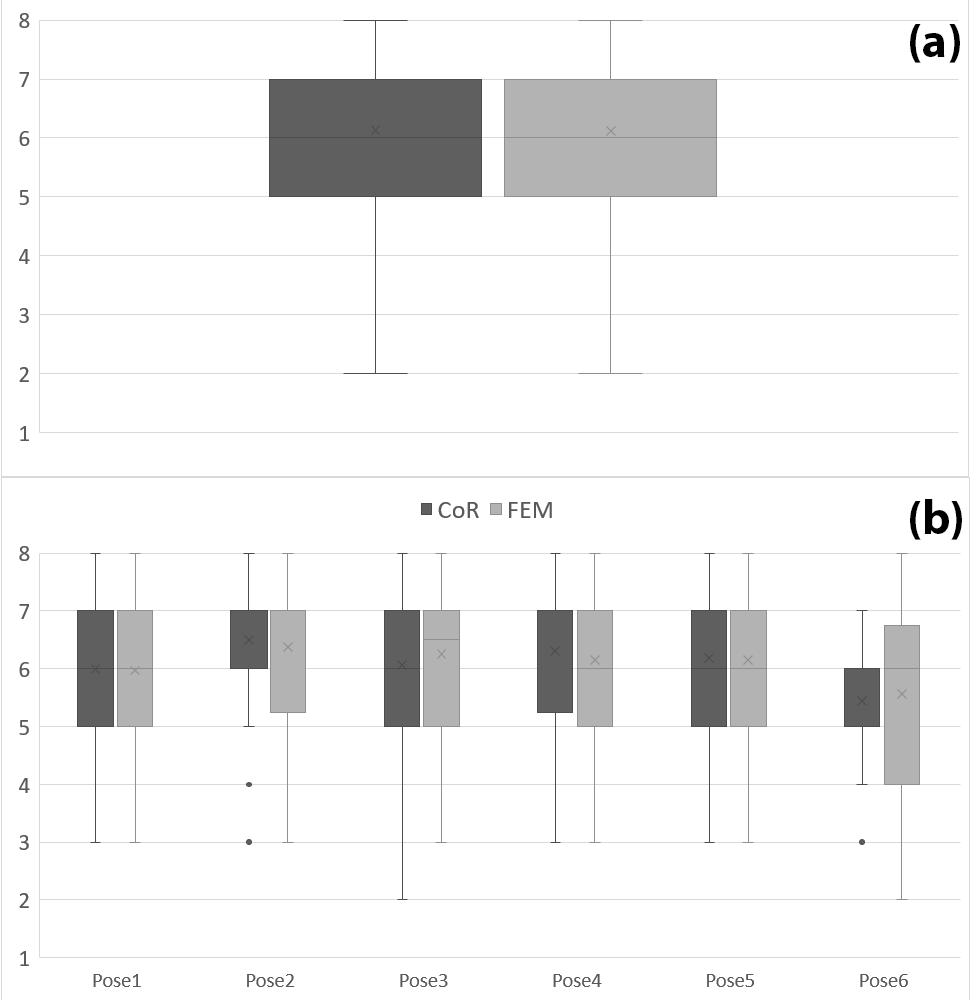
\includegraphics[width=0.45\textwidth]{IMG/boxplot}
    \caption{ Gráficas de cajas de bigotes comparando los resultados de la encuesta. Gráfica (a) muestra el resultado global, mientras la gráfica (b) compara el resultado obtenido por cada pose diferente.}
\label{fig:stat}
   \end{figure}

%%%%%%%%%%%%%%%%%%%%%%%%%%%%%%%%%%%%%

\subsection{ Animación de representaciones volumétricas}

\begin{figure*}[!ht]%[b]%[b!ht]
   \centering
   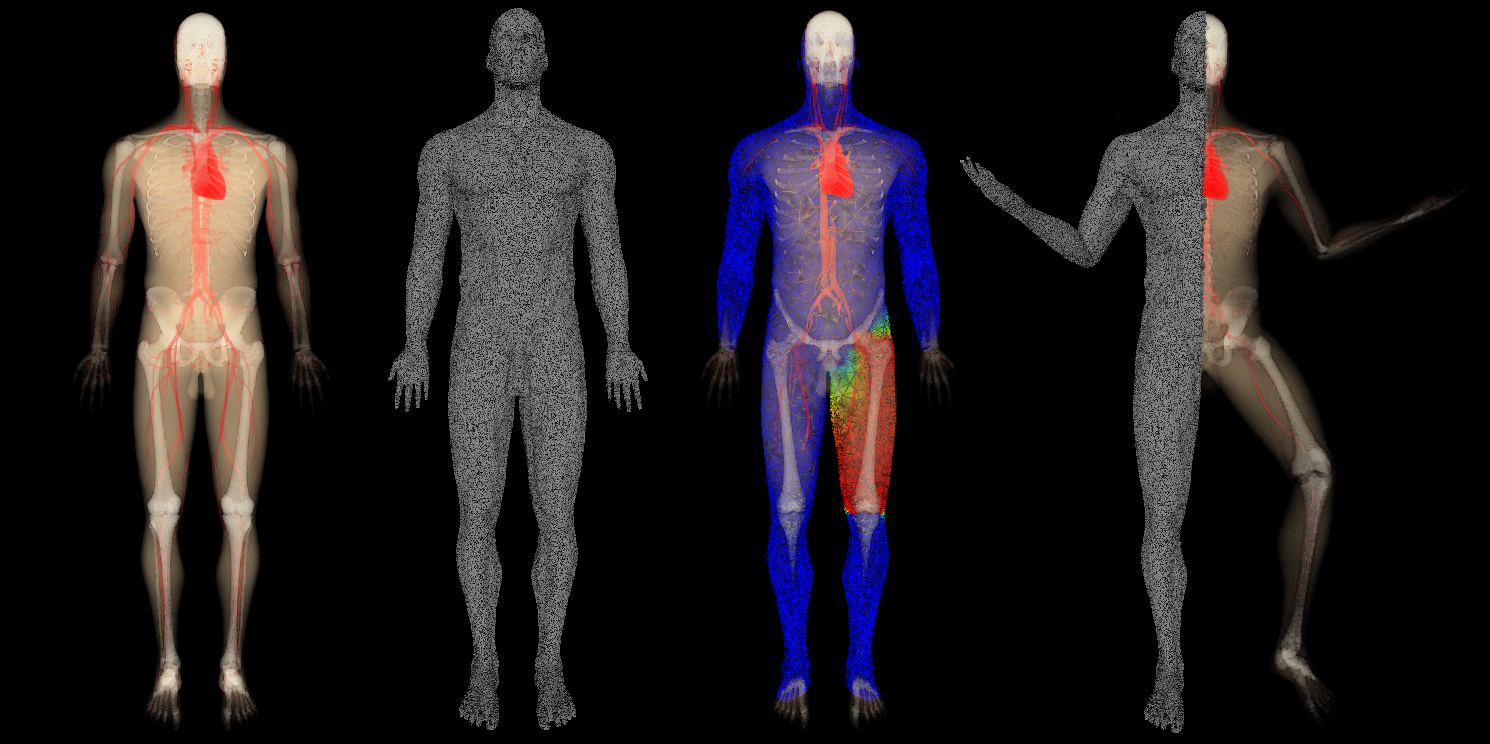
\includegraphics[width=0.90\textwidth]{IMG/Volumetric}
    \caption{Proceso de animación para modelo volumétrico. De izquierda a derecha: (1) modelo volumétrico en reposo, (2) malla de tetraedros generada, (3) malla de tetraedros representando el peso del fémur como ejemplo (rojo significa influencia cerca de 1, azul influencia 0) y (4) malla de tetraedros superpuesta al modelo volumétrico deformado. }
    \label{fig:volEx}
\end{figure*}
\todo{explica el por qué: el campo de desplazamientos}
La figura \ref{fig:volEx} muestra como puede ser utilizado el algoritmo propuesto a representaciones volumétricas de pacientes virtuales. En vez de transferir los pesos directamente de los tetraedros a los vértices interiores de los tejidos, se define un campo de desplazamientos que se puede usar para transformar tanto vértices de representaciones superficiales como para usarlo con \emph{vóxeles}. En este último caso, se definen una serie de \emph{píxeles} dentro de cada tetraedro en la posición deformada. Después son mapeados a la configuración de reposo utilizando la transformación inversa del campo de desplazamiento. Se itera sobre cada caja contenedora de la \ac{tabla hash} y se utilizan las coordenadas baricéntricas. Este proceso al ser fácilmente paralelizable en \ac{GPU} permite que se pueda \emph{renderizar} en tiempo real.
%


%%%%%%%%%%%%%%%%%%%%%%%%%%%%%%%%%%%%%
\begin{figure}[!ht]%[h]%[b]
   \centering
   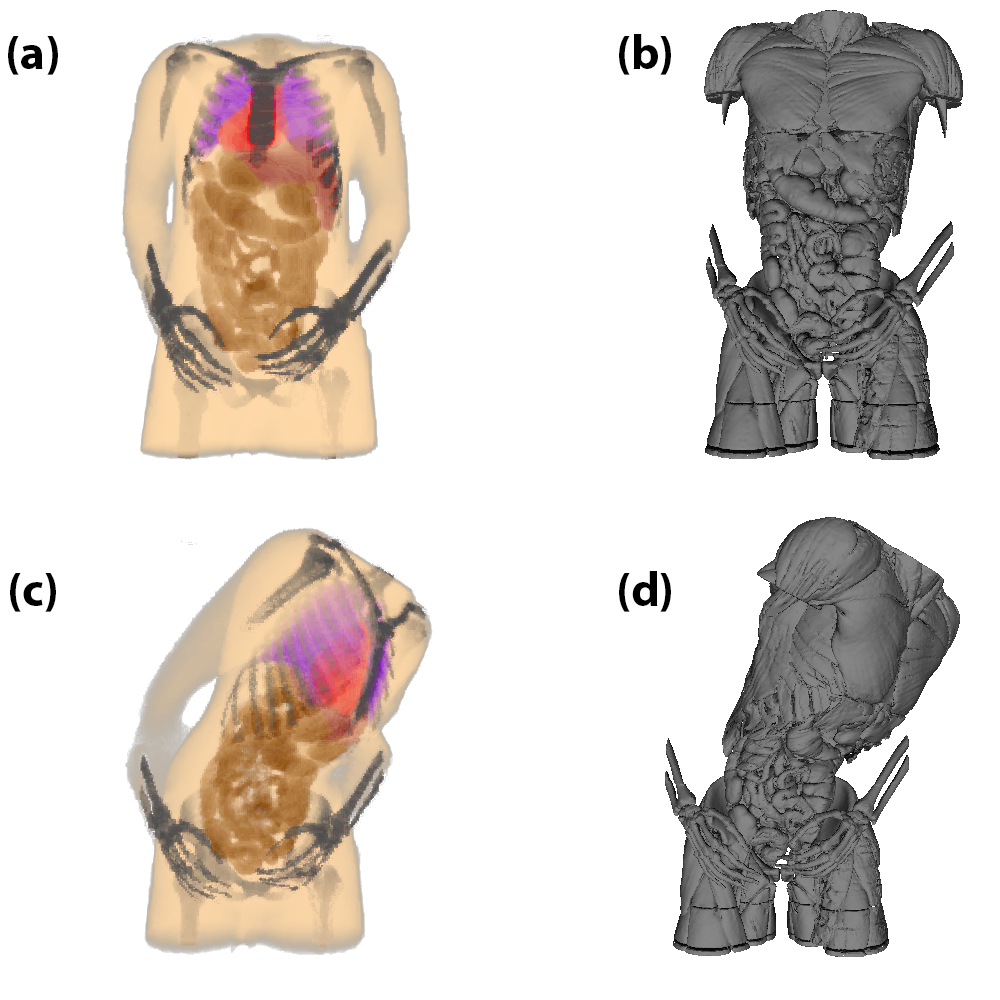
\includegraphics[width=0.4\textwidth]{IMG/HV}
    \caption{Algoritmo aplicado a diferentes representaciones: volumétrica (a) y (c), superficial (b) y (d). Imágenes (a) y (b) muestran el \emph{Segmented Inner Organs} en posición de reposo. Imágenes (c) y (d) muestran el resultado del modelo deformado.}
    \label{fig:humanvisible}
\end{figure}
Con la intención de seguir mostrando las capacidades del algoritmo propuesto, se presentan más ejemplos de deformaciones realizadas para esta tesis. En la figura \ref{fig:humanvisible} podemos observar tanto el modelo superficial como el volumétrico de los datos del proyecto \emph{Segmented Inner Organs}(\cite{VM2002},~\cite{VoxelMan}).



%%%%%%%%%%%%%%%%%%%%%%%%%%%%%%%%%%%%% 








%Due to their high content of water, organic tissues can be considered incompressible. For that reason, volume conservation is a desirable feature. In this vein, we have compared the behaviour of LBS, DQS, CoR and our Optimization step (FEM). To this end, we used the same MoCap walk cycle to animate the previously mentioned models. The results of this test are shown in Fig.  \ref{fig:volRatio}.
%\textcolor{red}{It can be observed how the optimization stage solve the volume problems of LBS and DQS. VER QUE PASA CON COR. }
%\begin{figure*}%[!ht]
%   \centering
%    \includegraphics[width=0.98\textwidth]%{img/graficas}
%    \caption{Volumen conservation rate of %the several \emph{skinning} techniques. }
%     \label{fig:volRatio}
%\end{figure*}

\section{Discusión}
\label{posing:discusion}
\todo{Hablar de la necesidad de validación}


\todo{La palabra realista me suena poco cientifica. Plausibles es un resultado que un usuario pueda interpretar como real.  }
\del{A la vista de los resultados, se puede afirmar que el algoritmo propuesto cumple con la función de generar resultados visualmente \del{realistas}\new{plausible} que en el contexto de entrenamiento puede ser utilizadas para que la transferencia de habilidades de los simuladores que la utilicen sea efectiva. } \todo{Como puedes afirmar que estos resultados son validos para el entrenamiento!!!!!!!! Has entrenado a médicos y después lo has evaluado!!!!! Aaron cuidado con lo que pones. La hipótesis es esa porque el objetivo era probar este sistema en herramientas reales. Hasta que no haya resultados en un simulador la hipótesis no queda probada!!!!!}

Esta técnica permite generar una cantidad infinita de variaciones anatómicas de un mismo modelo. En ese sentido, esta herramienta va a ser utilizada para crear una base de datos de modelos virtuales que posteriormente podrá ser utilizada tanto por el proyecto \ac{RASimAs}, como por aquellos simuladores que puedan beneficiarse del reposición de modelos anatómicos que permite el algoritmo propuesto. En el capítulo siguiente, se describirá como se ha incluido la solución presentada en el desarrollo de la herramienta \ac{TPTVPH}.

Por otra parte, la técnica presentada en esta tesis también puede cumplir con la funcionalidad de animar pacientes virtuales en herramientas interactivas. Este método se puede incorporar en cualquier simulador que requiera cambiar la pose a un determinado modelo anatómico con estructuras internas en tiempo real. Para demostrar esta funcionalidad, se presentará en los capítulos siguientes un simulador de radiología diagnóstica que utiliza las ventajas del modelo propuesto.

\new{El algoritmo propuesto se diseñó con el objetivo de ser lo más flexible posible, minimizando los requisitos de los datos de entrada. La clave de está flexibilidad radica en que se calcula un campo de deformaciones interno. Este campo de deformaciones permite adaptar cualquier tejido a la pose deseada, de forma independiente al resto de tejidos, pudiendo así trabajar con modelos incompletos. En este sentido, la única limitación es que tanto la piel como el tejido oseo del paciente virtual deben de estar segmentados. Esta restricción no supone un gran problema dado que estos tejidos son visibles en la mayor parte de las técnicas de imagen médica.}

\new{La flexibilidad que aporta el calculo del campo interno de deformaciones, aporta beneficios adicionales. Tal y como se muestra en la sección \ref{XXXXX}, este campo puede aplicarse a estructuras representadas tanto mediante B-reps \todo{mete acrónimo} como datos volumétricos. Extendiendo de esta manera el alcance de la técnica propuesta. }

\new{Evitar colisiones y autocolisiones en los tejido transformados es de vital importancia de cara a garantizar el buen funcionamiento del simulador físico y del simulador de \ac{US} de \ac{RASimAs}. Con el objetivo de garantizar este requisito, el algoritmo propuesto calcula un campo de deformaciones continuo. De esta forma, solo podrán aparecer colisiones y/o autocolisiones si: (i) se utilizan mallas para representar los tejidos con una resolución inadecuada o (ii) si existen colisiones y/o autocolisiones en el modelo virtual de partida. Debido a que la extracción de los tejidos desde imágenes médicas no es perfecta, pueden aparecer las auto colisiones y colisiones entre tejidos. La técnica propuesta no solventa estas colisiones, pero es robusta en su tratamiento. Aun así, las colisiones con el tejido oseo y muy especialmente con la piel, pueden provocar una importante perdida de realismo. Cabe destacar, que, a pesar de esta circunstancia, la técnica propuesta es mucho más robusta, en este escenario, que los métodos basados en simulación física. En la sección \ref{XX}, se proponen técnicas para mitigar estos problemas.}






%\appendix
%\include{appendix}
\cleardoublepage
% Como incorporar como un capitulo mas en el indice de la bibliografia
\addcontentsline{toc}{chapter}{Bibliografía}
\bibliography{bibliography}
\bibliographystyle{alpha}
\end{document}
